%%%%%%%%%%%%%%%%%%%%%%%%%%%%%%%%%%%%%%%%%
% Masters/Doctoral Thesis
% LaTeX Template
% Version 1.43 (17/5/14)
%
% This template has been downloaded from:
% http://www.LaTeXTemplates.com
%
% Original authors:
% Steven Gunn
% http://users.ecs.soton.ac.uk/srg/softwaretools/document/templates/
% and
% Sunil Patel
% http://www.sunilpatel.co.uk/thesis-template/
%
% License:
% CC BY-NC-SA 3.0 (http://creativecommons.org/licenses/by-nc-sa/3.0/)
%
% Note:
% Make sure to edit document variables in the Thesis.cls file
%
%%%%%%%%%%%%%%%%%%%%%%%%%%%%%%%%%%%%%%%%%

%----------------------------------------------------------------------------------------
%	PACKAGES AND OTHER DOCUMENT CONFIGURATIONS
%----------------------------------------------------------------------------------------

\documentclass[11pt, oneside]{Thesis} % The default font size and one-sided printing (no margin offsets)

\graphicspath{{pictures/}} % Specifies the directory where pictures are stored

\usepackage{titlesec}
\usepackage{todonotes}
\usepackage{pdfpages}
\usepackage{enumitem}

\titlespacing\section{0pt}{12pt plus 4pt minus 2pt}{0pt plus 2pt minus 2pt}
\titlespacing\subsection{0pt}{12pt plus 4pt minus 2pt}{0pt plus 2pt minus 2pt}
\titlespacing\subsubsection{0pt}{12pt plus 4pt minus 2pt}{0pt plus 2pt minus 2pt}

\setlength{\footnotesep}{0.3cm}
\setlength{\skip\footins}{1cm}

\usepackage[square, numbers, comma, sort&compress]{natbib} % Use the natbib reference package - read up on this to edit the reference style; if you want text (e.g. Smith et al., 2012) for the in-text references (instead of numbers), remove 'numbers'
\title{\ttitle} % Defines the thesis title - don't touch this

%----------------------------------------------------------------------------------------
%	MAIN DOCUMENT CONTENTS AND FRONT MATTER
%----------------------------------------------------------------------------------------

\begin{document}

\frontmatter % Use roman page numbering style (i, ii, iii, iv...) for the pre-content pages

\setstretch{1.3} % Line spacing of 1.3

% Define the page headers using the FancyHdr package and set up for one-sided printing
\fancyhead{} % Clears all page headers and footers
\rhead{\thepage} % Sets the right side header to show the page number
\lhead{} % Clears the left side page header

\pagestyle{fancy} % Finally, use the "fancy" page style to implement the FancyHdr headers

\newcommand{\HRule}{\rule{\linewidth}{0.5mm}} % New command to make the lines in the title page

% PDF meta-data
\hypersetup{pdftitle={\ttitle}}
\hypersetup{pdfsubject=\subjectname}
\hypersetup{pdfauthor=\authornames}
\hypersetup{pdfkeywords=\keywordnames}

%----------------------------------------------------------------------------------------
%	TITLE PAGE
%----------------------------------------------------------------------------------------

\begin{titlepage}
\begin{center}

\vspace*{3cm}

\HRule \\[0.4cm] % Horizontal line
{\huge \bfseries \ttitle}\\ %[1cm] % Thesis title
\HRule \\[1.5cm] % Horizontal line

\Large{\textsc{Bachelor Degree Thesis}}\\[3cm] % Thesis type

\begin{minipage}[t]{0.45\textwidth}
	\begin{flushleft} \large
		\emph{Author:}\\
		\authornames % Author name - remove the \href bracket to remove the link
		\vspace{1cm}
	\end{flushleft}
\end{minipage}
\begin{minipage}[t]{0.45\textwidth}
	\begin{flushright} \large
		\emph{Supervisor:} \\
		\supname\\ % Supervisor name - remove the \href bracket to remove the link
		\emph{Department:}\\
		\textsc{\supdept}
	\end{flushright}
\end{minipage}\\[2.5cm]

\Large \textsc{\degreename}\\
\large \textit{\textsc{\major}}\\[1cm] % University requirement text
%\textit{in the}\\[0.4cm]
%\groupname\\\deptname\\[2cm] % Research group name and department name

\textsc{\large \facname}\\ % University name
\textsc{\large \univname}\\[1cm] % University name

{\large \today}\\ % Date
%\includegraphics{Logo} % University/department logo - uncomment to place it

\vfill
\end{center}

\end{titlepage}

\clearpage % Start a new page
         % Thesis title page
%----------------------------------------------------------------------------------------
%	QUOTATION PAGE
%----------------------------------------------------------------------------------------

\pagestyle{empty} % No headers or footers for the following pages

\null\vfill % Add some space to move the quote down the page a bit

\textit{``Al fin y al cabo, somos lo que hacemos para cambiar lo que somos."}

\begin{flushright}
Eduardo Galeano
\end{flushright}

\vfill\vfill\vfill\vfill\vfill\vfill\null % Add some space at the bottom to position the quote just right

\clearpage % Start a new page
         % Remarkable quotation, by someone you like
%----------------------------------------------------------------------------------------
%	ABSTRACT PAGE
%----------------------------------------------------------------------------------------

\addtotoc{Abstract} % Add the "Abstract" page entry to the Contents

\abstract{\addtocontents{toc}{\vspace{1em}} % Add a gap in the Contents, for aesthetics

The Thesis Abstract is written here (and usually kept to just this page). The page is kept centered vertically so can expand into the blank space above the title too.
}

\clearpage % Start a new page
          % Thesis abstract
%----------------------------------------------------------------------------------------
%	ACKNOWLEDGEMENTS
%----------------------------------------------------------------------------------------

\setstretch{1.3} % Reset the line-spacing to 1.3 for body text (if it has changed)

\acknowledgements{\addtocontents{toc}{\vspace{1em}} % Add a gap in the Contents, for aesthetics

First and foremost, I would like to thank Dr. Jordi Nin for his advice and guidance throughout the entire development of this project, as well as his continued support to help me achieve my present and future goals. To him and all the professors I ever had, I am grateful of their will to teach and share their knowledge and sapience with all of us students; it is a great task you carry on your shoulders and for that you have my heartfelt gratitude.

Thanks to all inLab\textit{'ers} too. There, I have grown as an engineer and, most importantly, as a person, surrounded by amazing people. Thanks to Rosa, Albert and Jaume for their guidance, and thanks to all with whom I have had the most enthralling experiences at the faculty: Albert, Anna, Carlos, Eli, Germán, Jaume, Joel, Maki, Marc, MJ, Natxo, Néstor, and sure I forget someone.

I am most thankful to my dearest friends Bernat, Borja, Laura, Natàlia, Pau; all these years have been amazing by your side. With you, life is brighter and the future is always awaiting on the horizon.

This project would not be without my family. All my gratitude and love is for my parents and my brother, who support me and raise me and teach me the most wonderful things. Thank you.

}
\clearpage % Start a new page
  % Acknowledgements (family, friends...)
%----------------------------------------------------------------------------------------
%	LIST OF CONTENTS/FIGURES/TABLES PAGES
%----------------------------------------------------------------------------------------

\pagestyle{fancy} % The page style headers have been "empty" all this time, now use the "fancy" headers as defined before to bring them back

\lhead{\emph{Contents}} % Set the left side page header to "Contents"
\tableofcontents % Write out the Table of Contents

\lhead{\emph{List of Figures}} % Set the left side page header to "List of Figures"
\listoffigures % Write out the List of Figures

\lhead{\emph{List of Tables}} % Set the left side page header to "List of Tables"
\listoftables % Write out the List of Tables
            % TABLE OF CONTENTS, figures, tables, listings...
%----------------------------------------------------------------------------------------
%	ABBREVIATIONS
%----------------------------------------------------------------------------------------

\clearpage % Start a new page

\setstretch{1.5} % Set the line spacing to 1.5, this makes the following tables easier to read

\lhead{\emph{Abbreviations}} % Set the left side page header to "Abbreviations"
\listofsymbols{ll} % Include a list of Abbreviations (a table of two columns)
{
\textbf{DR} & \textbf{D}isclosure \textbf{R}isk \\
\textbf{IL} & \textbf{I}nformation \textbf{L}oss \\
\textbf{MOA} & \textbf{M}assive \textbf{O}nline \textbf{A}nalysis \\
\textbf{SDC} & \textbf{S}tatistical \textbf{D}isclosure \textbf{C}ontrol \\
%\textbf{Acronym} & \textbf{W}hat (it) \textbf{S}tands \textbf{F}or \\
}
     % Abbreviations used throughout the thesis
%----------------------------------------------------------------------------------------
%	SYMBOLS
%----------------------------------------------------------------------------------------

\clearpage % Start a new page

\lhead{\emph{Symbols}} % Set the left side page header to "Symbols"

\listofnomenclature{lll} % Include a list of Symbols (a three column table)
{
$a$ & distance & m \\
$P$ & power & W (Js$^{-1}$) \\
% Symbol & Name & Unit \\

& & \\ % Gap to separate the Roman symbols from the Greek

$\omega$ & angular frequency & rads$^{-1}$ \\
% Symbol & Name & Unit \\
}
           % List of symbols used
%----------------------------------------------------------------------------------------
%	DEDICATION
%----------------------------------------------------------------------------------------

\setstretch{1.3} % Return the line spacing back to 1.3

\pagestyle{empty} % Page style needs to be empty for this page

\dedicatory{Dedicated to my family.} % Dedication text

\addtocontents{toc}{\vspace{2em}} % Add a gap in the Contents, for aesthetics
        % Dedication oneliner

%----------------------------------------------------------------------------------------
%	THESIS CONTENT - CHAPTERS
%----------------------------------------------------------------------------------------

\mainmatter % Begin numeric (1,2,3...) page numbering

\pagestyle{fancy} % Return the page headers back to the "fancy" style

% Include the chapters of the thesis as separate files from the Chapters folder
% Uncomment the lines as you write the chapters

\chapter{Introduction} % Main chapter title
\label{Chapter1Introduction} % For referencing the chapter elsewhere, use \ref{Chapter1Introduction}
\lhead{\emph{Introduction}} % This is for the header on each page - perhaps a shortened title

%----------------------------------------------------------------------------------------

What follows is a brief introduction to the project under review in this report and its context,
in a broad sense. The structure of this document is also outlined in the last section of this chapter.

\section{Context}
\label{Introduction::Context}

We will now provide an overview of the two main concepts that, when combined,
drive the motivation behind the inception and development of this project.

\subsection{Data mining}
\label{Introduction::Context::DataMining}

Information society produces vast amounts of data all over the world.
This data comes from innumerable sources and in diverse formats, and has been stored
for years in data warehouses, waiting to be processed. With the continuous increase
in computing power, due to the recent advances in software and hardware technologies,
the machine learning field, more commonly known as \textit{data mining}, has arisen,
allowing us to exploit this stored data and distill knowledge from it.

Data mining is, indeed, a holistic process, where many different disciplines are
involved, from data acquisition and storage, through its selection, filtering and
analysis up to information extraction, visualization and knowledge discovery.

\begin{figure}[h]
	\centering
	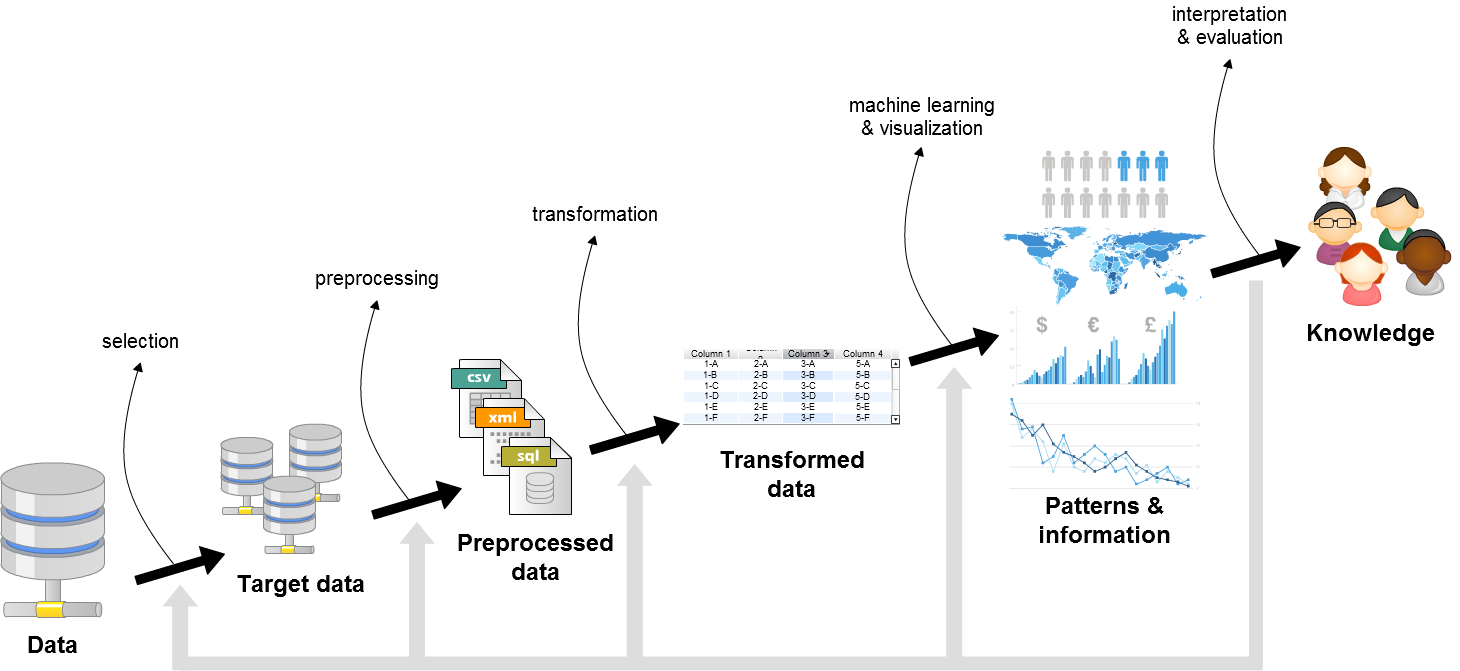
\includegraphics[width=0.9\linewidth]{figures/data-mining-process.png}
	\caption{Data mining as a process. Adapted from~\citet{Fayyad:FromDataMining}}
	\label{fig:data-mining}
\end{figure}

Data mining enables a better understanding of human or natural processes and provides
us with means to identify trends, predict future events or discover useful patterns.
Its uses range from scientific and medical applications to social sciences or business
administration~\citep{Fayyad:FromDataMining}.

\subsubsection{Facing the limits}

Despite lots of effort is put into enhancing different data mining processes, there still
are many cases where these techniques fail to perform correctly; mainly, it is a matter of scale.

On one hand, traditional data mining workflows cannot cope with the really massive
data sets that are available nowadays, if performed on a common infrastructure.
To solve this issue, clusters of hundreds or thousands of computers are used to run
such analysis. It is costly and complex but, doing so, we can mine data that we could not
some time ago.

On the other hand, we face another type of scaling problem. In some situations, data
acquisition throughput is so high that it cannot be stored anyway, so another approach
is needed to avoid the loss of information that it could deliver us. Moreover, we might
not want to store it, even when we could, but yet we want to analyze it to extract
knowledge from it, as soon as we received it. Both these scenarios are addressed with a
series of techniques known as \textit{stream mining}.

\subsubsection{Stream mining}

\textit{Stream mining} or \textit{data stream mining} is a process that allows us to
still discover knowledge and patterns in data, even when it comes in the form of a
continuous stream, or many of them~\citep{Rajaraman:MiningMassiveDatasets}. Instead of processing
all statically stored data, like traditional data mining does, a relatively small
portion of it is kept during the analysis, and it is updated when needed - either because
more resources are available to the system or because new data is acquired. A more deeper
review of this research area is given in \ref{Theory::StreamMining}.

\subsection{Privacy}
\label{Introduction::Context::Privacy}

Privacy is a concept that can be defined as the ability of an individual or group to
seclude\footnote{“Seclusion is the act of placing or keeping someone away from other people.”~\citep{web:Merriam:Seclusion}} themselves, or information about themselves, and
thereby express themselves selectively. It is understood differently depending on the social
and cultural background of each individual, but it is in fact recognised as one of the most
fundamental rights of our human nature. The Universal Declaration of Human Rights’ 12th
article~\citep{web:UN:HumanRightsDeclaration} states that:

\begin{quote}
	No one shall be subjected to arbitrary interference with his privacy, family, home or
	correspondence, nor to attacks upon his honour and reputation. Everyone has the right to
	the protection of the law against such interference or attacks.
\end{quote}

This right has been continuously violated ever since information exchange and advanced
communication technologies have been developed. Despite this did not begin with the spread
of the Internet, its adoption has greatly magnified both the ability to breach people’s privacy
and the impact that these breaches have. A more thorough analysis of privacy and its interrelations
with society and technology is given in \sref{Practical::Privacy}.

\subsection{Privacy Preserving Data Mining}
\label{Introduction::Context::PPSM}

Data mining technologies have become a relevant debate topic nowadays, concerning what
information is collected from individuals, who owns it and what are the purposes behind
its gathering. Information technologies deliver us many benefits at many levels - safer
streets, cheaper communications, better health systems, more convenient shopping - but
at the high cost of losing our privacy.

Knowledge discovery processes need data to work and, in most cases, it is sensitive and
personal. Moreover, it is massively collected and stored and analyzed without us knowing
much about it. Besides the lack of consent in this data acquisition stage of the process,
data mining poses a bigger thread on individuals: information disclosure. Sensitive data
must be treated accordingly, which involves not only good IT security practices to avoid
information leaks, but a responsible treatment when research results are published.

\subsubsection{Statistical Disclosure Control}

\textit{Statistical Disclosure Control} (SDC) is the name that the statistical community
has given to what the data mining community calls Privacy Preserving Data Mining (PPDM).
This field, whatever its preferred name is, deals with controlling that information about
specific individuals is not extracted from statistical summary results. Also, if full
datasets are to be released, PPDM methods should be applied to data in order to preserve
user's privacy, whilst maintaining the statistical significance of it, i. e., the amount
of information - knowledge - that this data can provide.

\section{The project: moa-ppsm}
\label{Introduction::moa-ppsm}

Having reviewed the main concepts to which this project is related, we can now outline
its main purpose, once we take a closer look to the technical environment in which it
will be developed.

\subsection{MOA}
\label{Introduction::moa-ppsm::MOA}

\textbf{MOA}, initials for \textbf{M}assive \textbf{O}nline \textbf{A}nalysis, is an
open source framework for data stream mining~\citep{web:MOA}, originally
developed at the University of Waikato, New Zealand. It includes several machine learning
algorithms\footnote{Algorithms used to perform the actual data mining analysis (the
“machine learning \& visualization” step on \fref{fig:data-mining}) belong to the
field of machine learning. In MOA, clustering, classification, regression, outlier
detection and recommender systems are available.} to perform the analysis and tools
to evaluate the quality of the results. It also deals with a problem known as
\textit{concept drift}\footnote{It is said of statistical properties of a target variable
being analyed, when they change over time in unforeseen ways.}. It is related to the well
known and commonly used Weka\footnote{Weka is a popular software package including
classical data mining algorithms, this is, not stream mining. It is also developed at
the University of Waikato.~\citep{web:Weka}} package, but it is built to perform at
a greater scale for more demanding problems.

\begin{figure}[h]
	\centering
	
\includegraphics[width=0.4\linewidth]{figures/moa-logo.jpg}
	\caption{Massive Online Analysis logo.}
	\label{fig:moa-logo}
\end{figure}

\subsubsection{MOA filters}

One of the available features in MOA is the use of \textit{filters}, which can process
streaming data before or after being fed to other systems or algorithms, such as learners
or file writers. However, few filters are currently shipped within the latest MOA distribution,
namely a filter to replace \textit{missing values}\footnote{In statistics, missing data, or missing values,
occur when no data value is stored for the variable in an observation. Missing data are a
common occurrence and can have a significant effect on the conclusions that can be drawn
from the data.} and a filter that adds noise to data.

\subsubsection{MOA extensions}

When working with MOA, the environment consists of the core library, but \textit{extensions}
can be used to enhance the existing methods or to provide additional features, based on
the core tools that MOA already provides. A series of extensions have been developed and can
be found on MOA's website, at \url{http://moa.cms.waikato.ac.nz/moa-extensions}.

\subsection{The project in a nutshell}
\label{Introduction::moa-ppsm::ProjectNutshell}

Summing up, the aim of this project is to \textbf{implement privacy preserving filters
for the MOA stream mining framework}. This is, adapt some well-known SDC methods to a stream mining environment and, more precisely, to the MOA software framework, in the form of a MOA extension.

\section{Report structure}
\label{Introduction::Structure}

The structure of this report is meant to give an overview of the development process of the project, from the theoretical foundations that are necessary to understand the work to the final results and conclusions.

\cref{Chapter2TheoreticalFramework} covers the theory basis behind the SDC methods implemented in the project and provides some insights on different stream mining approaches. \cref{Chapter3StateOfTheArt} discusses state of the art solutions concerning SDC for static databases (not streaming data). \cref{Chapter4PracticalAspects} analyzes more thoroughly the motivation behind privacy-preserving data mining by discussing \textit{practical} questions like the relationship between society and privacy or the legal framework that applies to the context of this project. Project management is layed out in \cref{Chapter5ProjectManagement} and then the report turns to more technical related topics, such as implementation details and desgin decisions, covered in \cref{Chapter6ImplementingFilters}, as well as benchmarking, in \cref{Chapter7Benchmarking}. Finally, the report and project conclusions are given in \cref{Chapter8conclusions}, covering both achievements and possible future work.

\chapter{Theoretical framework} % Main chapter title
\label{Chapter2TheoreticalFramework} % For referencing the chapter elsewhere, use \ref{Chapter1Introduction}
\lhead{\emph{Theoretical framework}} % This is for the header on each page - perhaps a shortened title

%----------------------------------------------------------------------------------------

\todo{write an appropriate intro to theoretical framework}
What follows is a brief introduction to the project under review in this report and its context,
in a broad sense. The structure of this document is also outlined in the last section of this chapter.

\section{Stream Mining}
\label{Theory::StreamMining}

Data stream mining is a relatively new field. Even though its theoretical foundation is based in well-established statistical and computational approaches, it has not been until recent years that this research area has experimented a great growth in interest.

The main problem when dealing with streaming data is the high throughput of data being analyzed, under computational resources constraints. Variable data rates is another problem that has to be addressed too. Once these problems are resolved, the same kind of data mining analysis as in the case of batch data processing are available: classification, regression or clustering tasks, as well as outlier detection and recommendation systems. We will not cover these techniques here, because they are not related to this project, by themselves. Instead, we will have a look at some different stream mining solutions, because their working principles do affect the way the project’s algorithms will be implemented.

\subsection{Stream mining approaches}
\label{Theory::StreamMining::Approaches}

Solutions provided in this field can be categorized into \textit{data-based} and \textit{task-based} ones~\citep{Gaber:MiningDataStreamsReview}, depending on their approach.

\subsubsection*{Data-based stream mining solutions}

The idea behind these solutions is to use a subset of the original dataset to perform the required analyses. Diverse techniques that have been used in this sense can further be split into two more categories:

\begin{itemize}
	\item \textbf{Sampling methods:} either by randomly picking samples of the data stream or by randomly selecting chunks (subsets) of the stream, sampling methods discard part of the incoming data, while performing the knowledge discovery processes with the sampled data. The main problem with this approach is that is hard to know when to pick a sample or which records should be stored, because there is no previous knowledge of the dataset size or its information structure.

	\item \textbf{Summarizing methods:} they use aggregated data or calculated statistical measures (that are continuously recalculated) to provide the information needed for the data mining algorithms. In this case, it is the loss of information and accuracy and the inability to control data distribution fluctuations what renders these methods not so usable as it was desired.
\end{itemize}

\begin{figure}
\centering
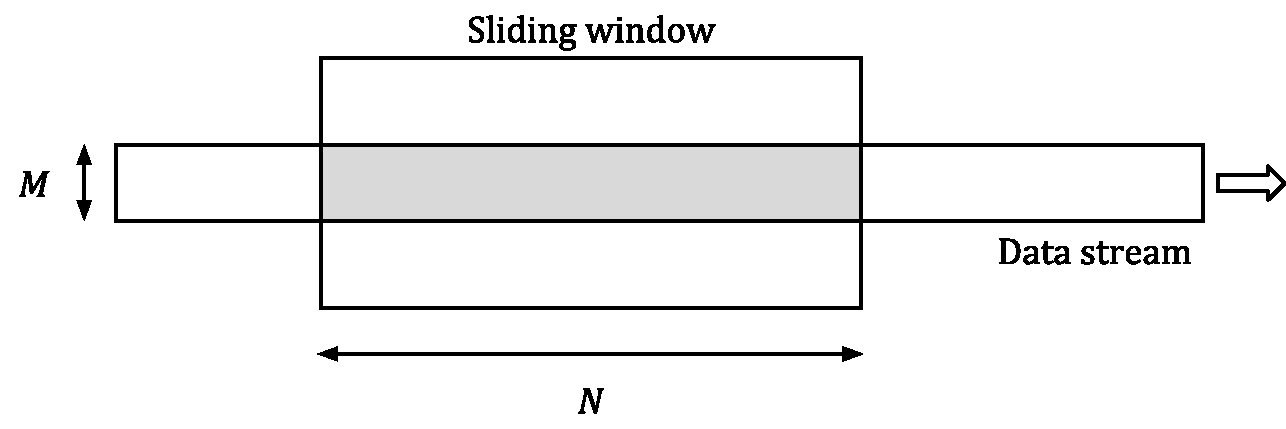
\includegraphics[width=0.9\linewidth]{figures/sliding-window.pdf}
\caption[Sliding window based stream processing.]{Processing a data stream using a \textit{sliding window} approach. In the figure, $N$ is the \textit{size} of the sliding window, in terms of the number of samples of the stream being stored, whereas $M$ is the number of \textit{attributes} of the samples in the stream.}
\label{fig:sliding-window}
\end{figure}

\subsubsection*{Task-based stream mining solutions}

The solutions that fall into this category are based not on performing data transformations, but on changing the data mining methods to enable their use on data streams.

\begin{itemize}
	\item \textbf{Approximation algorithms:} these are a kind of algorithms that are designed to solve computationally hard problems, by giving an approximate result. Instead of computing exact solutions, they just guarantee a certain error bound. The problem with these methods is, again, the high received data throughput, which they cannot cope as well. Additional tooling is therefore needed if one wishes to use them.

	\item \textbf{Sliding window method:} this method, a common pattern in many online\footnote{In computer science, an \textit{online algorithm} is one that can process its input piece-by-piece in a serial fashion, i.e., in the order that the input is fed to the algorithm, without having the entire input available from the start.} applications, maintains a \textit{sliding window} in which the most recent data is kept. As data is received from the incoming streams, this window “advances” so new observations are kept inside, as can be seen in \fref{fig:sliding-window}. The data mining analyses are then performed using the data available inside the window and summarized versions of the older records, in the form of statistical measures or aggregated data.
	This particular method is the one that the MOA package uses - thus its name: Massive \textbf{Online} Analysis. This solution scheme enables dealing with concept drift, which would not be possible if just aggregated data was used.

	\item \textbf{Algorithm output granularity:} this method is a resource-aware data analysis approach that can perform the local analysis on resource constrained devices, by adapting to resource availability and data stream rates - when resources are completely running out, the results are merged and stored.
\end{itemize}

\section{Statistical Disclosure Control}
\label{Theory:SDC}

As was already introduced in \sref{Introduction::Context::PPSM}, the purpose of Statistical Disclosure Control (SDC) is to prevent confidential information from being linked to specific individuals to whom this data belongs. We will review now some concepts related to data disclosure and SDC methods and some theoretical foundations.

\subsection{Privacy preserving algorithms} 
\label{Theory:SDC:Algorithms}

As a quick and superficial review, the algorithms\footnote{We will not cover every algorithm in detail, because some of them are not included in the scope of this project.} being used nowadays to achieve effective privacy preserving in datasets can be categorized into the following groups~\cite{Hundepool:StatisticalDisclosureControl}:

\begin{itemize}
	\item \textit{Non-perturbative data masking:} these kind of methods do not perform data values transformations. Instead, they are based in partial suppressions of records or reductions of detail of the datasets. Some examples are:
	\begin{itemize}
		\item Sampling
		\item Global recoding
		\item Top and bottom coding
		\item Local suppression
	\end{itemize}

	\item \textit{Perturbative data masking:} these methods do release the whole dataset, if required, but it is perturbed, this is, values are changed by adding them noise. This way, records are diffused and reidentifying individuals is harder. Some examples are:
	\begin{itemize}
		\item Noise masking
		\item Micro-aggregation
		\item Rank swapping
		\item Data shuffling
		\item Rounding
		\item Re-sampling
		\item PRAM
		\item MASSC
	\end{itemize}
\end{itemize}

\subsection{Disclosure \& types of variables}
\label{Theory:SDC:DisclosureTypes}

When assessing the disclosure risks of a given dataset (or data stream) we must have a look at the different kind of variables this data is composed of. We will stick to a classic~\citep{Templ:IntroSDC} categorization of such attributes into three groups, which need not be disjunctive, as follows:

\begin{itemize}
	\item \textbf{Identifiers:} variables that precisely identify individuals, e.g., social insurance numbers, person names, or addresses.
	\item \textbf{Quasi-identifiers:} a set of variables that, when considered together, can be used to identify individual units. It might be possible to, for example, identify people by combining variables such as gender, age, region and occupation.
	\item \textbf{Non-identifying variables:} these are neither \textit{identifiers} nor \textit{quasi-identifiers}.
\end{itemize}

Concerning \textit{disclosure}, it is also defined differently depending on the type of privacy breach that has occurred:

\begin{itemize}
	\item We talk about \textit{identity disclosure} when a specific individual record can be recognised in a dataset, i.e., when linkage with external available data is possible. Identity disclosure is performed using direct identifiers, rare combinations of values in quasi-identifier attributes and exact knowledge of variable values in external databases.
	\item In the case of \textit{attribute disclosure}, the intruder is able to gather sensitive information about a specific unit from the released data, where it is directly available. For example, if no perturbation is applied to the original values of the \textit{wages} variable, one could learn how much a person is earning if its identity is disclosed too.
	\item \textit{Inferential disclosure}, the most general case, occurs when an intruder is able to, with some uncertainty, predict or \textit{infer} confidential information about an individual from the statistical properties of data.
\end{itemize}

It is important to remark that a subset of critical variables might be exploited to disclose every information about a single unit in a dataset. Thus, we are bound to carefully select which variables of the dataset might be released to further users of the data, while trying to maximize its statistical utility. More concretely, it is extremely important to \textbf{not release identifiers} and to analyze quasi-identifiers closely, in order to avoid information leaks and privacy breaches.

\subsection{Disclosure Risk}
\label{Theory:SDC:DiscRisk}

Concerning the safety of the released data, \textbf{Disclosure Risk} (DR) is a common way to measure and assess the risk of re-identification of particular individuals. Re-identification happens when some sensitive and confidential data that have been released are subsequently linked to a particular individual, which results in a confidentiality breach. There are a number of different approaches in how to assess disclosure risk and whether to measure it \textit{per record} or globally, taking into account the whole dataset.

As noted in \citep{Domingo:DiscRiskAssessment}, there is not much literature on disclosure risk that can be used for a broad class of perturbative methods; disclosure risk measures tend instead to be method-specific. Therefore, empirical methods are most used to assess disclosure risk for these kind of methods.

\subsubsection{Record linkage}

Most notably, the mechanisms used to measure disclosure risk follow a \textit{record linkage} approach. This is, after an SDC method has been used to anonymize data, a record linkage procedure is applied to the original and released (masked, anonymized) datasets. This \textit{linkage} attempts to identify, for each record in the masked dataset, which is the corresponding record in the original dataset. If such correspondance is verified, the record is labeled as \textit{correctly linked}. A generic measure for disclosure risk is the percentage of correctly linked records from the total amount in the dataset.

\begin{itemize}
	\item \textbf{Distance-based record linkage:} provided that a \textit{distance} measure can be defined between the original and the masked datasets, linkage is performed as follows: for each record in the anonymized dataset, a distance to each record in the original dataset is calculated. The nearest record, in terms of this distance measurement, is assumed to be the corresponding record, thus establishing a \textit{link} between them. This linkage is then verified to assess how many of these guesses are true re-identifications.
	
	\item \textbf{Probabilistic record linkage:} in this case, the matching algoritm works a little different. For each possible pair of original and masked records, a \textit{coincidence vector} is defined. This vector holds, for each attribute, whether or not the values of the considered records are equal. An index is computed afterwards over these vectors and, using such index, the records pairs are classified as \textit{linked} or \textit{not linked}. Again, this linkage is verified to assess the number of true re-identifications.
\end{itemize}

\subsection{Information Loss}
\label{Theory:SDC:InfoLoss}

Another key measurement concerning data protection is \textbf{Information Loss} (IL) or \textit{data utility}, which could be defined as the amount of useful statistical information that is lost along the data masking process. A good SDC method should try to minimize IL, in order to provide optimally useful data to the legitimate users of such data, while also keeping a low disclosure risk. It is important to note that these two properties are inversely proportional: the lower disclosure risk is, the higher information loss will occur. This trade off between these two parameters is often a difficult and challenging task and should be taken into very careful consideration, depending on the release policies that apply, the kind of data being released and the sensitivity of the information contained in such data. This evaluation should be performed not only from a purely quantitave and numerical point of view, but from an ethical and privacy concerned one too.

As well as with disclosure risk, a number of methods and approaches are taken to assess information loss when releasing privacy protected datasets, ranging from unbounded~\citep{Domingo:SDCMethodsInfoLoss} to probabilistic (bound to the $[0,1]$ interval) measurements~\citep{Mateo:ProbInfLossMeasures}.

\subsubsection*{Unbounded Information Loss}

An example framework to assess IL was given in \citep{Domingo:SDCMethodsInfoLoss}, which evaluates some key statistical properties of the released data. More concretely, it computes three \textit{discrepancy} measurements for a series of pairs of matrices (correlation, covariance, etc. of the original and masked datasets), namely the \textit{mean square error}, the \textit{mean absolute error} and the \textit{mean variation}.

\subsubsection*{Probabilistic Information Loss}

The aim of measuring IL in a probabilistic manner is to bound this measurement to the $[0,1]$ range, thus allowing its comparison with DR, which is also generally expressed within this range. This way, a \textit{score} could be calculated from both normalized measures for an SDC method, easing parameters selection to data protectors, for example.

\subsection{Privacy guarantees}
\label{Theory:SDC:Guarantees}

Many different methods have been developed to help prevent information disclosure when data mining datasets or results are released. These algorithms pursue the generation of results or data that have particular properties concerning privacy preservation. Some of the desirable properties of privacy-protected data are described in the following sections, but no formal definition is provided for some of them (please refer to the original papers and publications to understand them better).

\subsubsection{\textit{k}-Anonymity}

First described in 2002, by Latanya Sweeney, a release of data is said to have the \textit{$k$-anonymity} property if the information for each person contained in the release cannot be distinguished from at least $k-1$ individuals whose information also appears in the release~\citep{Sweeney:kAnonymity}. A more formal definition uses the previously reviewed concept of \textit{quasi-identifiers} (see~\sref{Theory:SDC:DisclosureTypes}).

\begin{definition}~($k$-Anonymity)
A dataset is said to satisfy $k$-anonymity for an integer $k > 1$ if, for each combination of values of quasi-identifiers, at least $k$ records exist in the dataset sharing that combination.~\citep{Domingo:EnhancingDiffPrivMicroaggregation}
\end{definition}

An intruder trying to use a $k$-anonymous dataset to do, for example, record linkage against an external source of information will find that at least $k$ records in the dataset match any value of the quasi-identifiers that he or she is trying to use to perform the linkage. Thus, re-identification is limited to \textit{groups}, this is, no individual records can be linked, just groups of size at least $k$.

\subsubsection{\textit{l}-Diversity}

The evolution of the concept of $k$-anonymity is \textit{$l$-diversity} and adds further privacy preservation by adding intra-group diversity, so to avoid the flaws of the $k$-anonymity privacy model~\citep{Machanavajjhala:lDiversity}.

\subsubsection{\textit{t}-Closeness}

Further on, the \textit{$t$-closeness} property definition adds attribute-based privacy enforcement to the $l$-diversity model: to better preserve privacy, all values (all observations) from a particular attribute must not be too much different - instead, they should be close up to a certain threshold~\citep{Ninghui:tCloseness}. This is needed to preserve the privacy of those records that are more easily identifiable because their attribute values are more distinguishable.

\subsubsection{Differential Privacy}

Described in~\citet{Dwork:DifferentialPrivacy}, \textit{differential privacy} is a condition \textit{on the release mechanism} (not the dataset) that guarantees a strong privacy preservation level for some particular data uses contexts. Differential privacy is introduced in an \textit{interactive} setting, i.e., in a query-response data retrieval environment, and offers probabilistic guarantees that the contribution of any single individual to thenquery response is limited.

\begin{definition}~($\varepsilon$-Differential privacy)
A randomized mechanism\footnote{By \textit{mechanism}, we refer to any kind of function or system used to query for data.} $\mathcal{M}$ gives $\varepsilon$-differential privacy if, for all datasets $X_1$, $X_2$ such that one can be obtained from the other by modifying a \textit{single} record, and all $S \subset Range(\mathcal{M})$, it holds
\begin{equation}
P(\mathcal{M}(X_1) \in S) \leq \mathrm{exp}(\varepsilon) \times P(\mathcal{M}(X_2) \in S)
\end{equation}
\end{definition}

This definition, cited from~\citet{Domingo:EnhancingDiffPrivMicroaggregation}, easier to understand than the original one given in~\citet{Dwork:DifferentialPrivacy}, states that, given an $\varepsilon$-differential privacy mechanism $\mathcal{M}$ and any possible output $r$, the presence or abscence of a participant (in terms of the dataset, a \textit{row}) will cause at most a multiplicative $e^\varepsilon$ change in the probability of the mechanism to output a response $r$.
\section{SDC methods}
\label{Theory:SDCMethods}

We will describe now some of the most common methods and mechanisms used in SDC applications to anonymize data or provide privacy preserving data releases.

\subsection*{Notation}

We assume the following notation for the subsequent method descriptions:

\begin{itemize}
	\item
	The original dataset is the matrix $X$, with $n$ rows (samples) and $m$ attributes or variables. Therefore, the $x_{ij}$ element of the dataset denotes the value that the $j$-th attribute takes in the $i$-th row for any $1 \leq i \leq n$ and $1 \leq j \leq m$.
	
	\item
	The anonymized (protected) dataset is named $X'$.
\end{itemize}

\subsection{Noise Addition}
\label{Theory:SDCMethods:NoiseAddition}

Noise addition or \textit{additive noise masking} is a fairly simple method that is based on the addition of gaussian noise to data, thus randomly distorting its values and difficulting re-identification of individuals. The main additive noise algorithms in the literature are~\citep[p. 54]{Hundepool:StatisticalDisclosureControl}:

\begin{itemize}
	\item
	Uncorrelated noise addition.
	\item
	Correlated noise addition.
	\item
	Noise addition and linear transformation.
	\item
	Noise addition and non-linear transformation.
\end{itemize}

We will only cover the first couple of methods, because of the inherent difficulty of the latter, both in its theoretical basis and its practical implementation, which renders them not suitable for the needs of this project.

\subsubsection{Uncorrelated noise addition}

Masking by additive noise the $j$-th variable of an original dataset $X$ yields an anonymized dataset $X'$ such that

\begin{equation}
x_{ij}' = x_{ij} + \epsilon\ \ \ \text{for}\ 1 \leq i \leq n
\end{equation}

where $\epsilon$ is drawn from a random variable $\varepsilon_j \sim N(0,\sigma_{\varepsilon_j}^2)$. The general assumption is that the variances of each $\varepsilon_j$ are proportional to those of the original variables, this is, if $\textrm{Var}(X_j) = \sigma_j^2$ is the variance of the $j$-th attibute of the dataset $X$, then $\sigma_{\varepsilon_j}^2 := \alpha\sigma_j^2$.

While this method preserves means and covariances, it is, unfortunately, not able to preserve variances nor correlation coefficients.

\subsubsection{Correlated noise addition}

This method is aimed to also preserve correlation coefficients, with respect to \textit{uncorrelated} noise addition. The main difference with the previous mechanism is that the covariance matrix of the errors is now proportional to the covariance matrix of the data: $\varepsilon \sim N(0,\Sigma_\varepsilon)$, where $\Sigma_\varepsilon = \alpha\Sigma$.

Masking by correlated noise addition provides data with higher analytical utility than masking using uncorrelated noise, as long as $\alpha$ is revealed to the data user. However, the low level of protection yielded by this method and the previous one render them as not very useful for truly important SDC applications.

\subsection{Microaggregation}
\label{Theory:SDCMethods:Microaggregation}

Originally described for continuous (numerical) data, microaggregation is a family of SDC methods that, in the most general form, consist of making homogeneous groups of $k$ or more individuals (rows) from within the $X$ dataset to later replace their values with aggregated ones, this is, averages, computed on the groups themselves. These grouped and aggregated records conform the resulting $X'$ release dataset.

Two main approaches are taken when considering microaggregation techniques: \textit{univariate} and \textit{multivariate} microaggregation. The difference remains in the number of variables used to perform the \textit{clustering} phase of the method: a single variable and multiple attributes, correspondingly. As can be assessed in the literature, the univariate approach causes either a very high information loss or a very high disclosure risk, thus not being appropriate for normal SDC uses~\citep[p. 63]{Hundepool:StatisticalDisclosureControl}. On the other hand, multivariate microaggregation, proposed by~\citet{Domingo:PracticalMicroaggregation}, is considered an excellent protection method and, as such, we will focus on this approach.

It is important to note that this family of techniques are directly related to $k$-anonymity, as proved in~\citet{Domingo:KAnonMicroagg}.

\subsubsection{Partition}

The first and most computational complex task to do in a microaggregation method is to partition the dataset into $g$ groups of size at least $k > 1$, which is, indeed, a \textit{clustering} task. This proves to be quite difficult, but an optimal solution approximation with respect to information loss was already given in~\citep{Domingo:KAnonMicroagg} and further refined in~\citet{Domingo:MuAproxPolyTimeMicroagg}.

The aim of these partition methods is to find the optimal $k$-partition that maximizes within-group homogeneity. Following~\citet{Domingo:PracticalMicroaggregation}, a practical information loss measure for microaggregation, relatively common in the clustering literature, is the ratio of within-group homogeneity over the total sum of squares (the sum of \textit{within} and \textit{between} group homogeneity)

\begin{equation}\label{eq:clustering-info-loss}
L = \frac{SSE}{SST}
\end{equation}

The within-group homogeneity ($SSE$) is defined as

\begin{equation}
SSE = \sum_{i=1}^{g} \sum_{j=1}^{n_i} (x_{ij} - \mathbf{\bar{x}_i})^2
\end{equation}

where $g$ denotes the total number of groups of $n_i$ elements each and $\mathbf{\bar{x}_i}$ denotes the $i$-th group centroid. The between-groups sum of squares, $SSA$, is

\begin{equation}
SSA = \sum_{i=1}^{g} n_i (\mathbf{\bar{x}_i} - \mathbf{\bar{x}})^2
\end{equation}

where $\mathbf{\bar{x}}$ is the average vector over the whole dataset. The total sum of squares is, then, $SST = SSE + SSA$.

Because microaggregation replaces values in a group by the group centroid, if we recall~\eref{eq:clustering-info-loss}, it follows that the higher the within-group homogeneity, the lower the information loss is. Both the MDAV~\citep{Domingo:KAnonMicroagg} (Maximum Distance to Average Vector) and $\mu$-Approx~\citep{Domingo:MuAproxPolyTimeMicroagg} algorithms are built to partition the dataset into groups, while minimizing information loss, exploiting the previous theoretical result.

\subsubsection{Aggregation}

The aggregation step is the simplest of the ones that take place in a microaggregation setting: for each group $g$ of at least $k$ records and for each attribute $1 \leq j \leq m$, an \textit{aggregate} $\gamma$ is computed among the values of the $j$-th variable for the records in the group. This aggregate is then imputed to each record for its $j$-th attribute.

Concerning the types of variables that are aggregated~\citep{Domingo:KAnonMicroagg}:

\begin{itemize}
	\item
	\textbf{Continuous attributes:} the aggregated value correponds with the arithmetical mean of the selected values.
	\item
	\textbf{Categorical attributes:} the aggregated value should either be the median or the mode of the selected values.
\end{itemize}

\subsection{Rank Swapping}
\label{Theory:SDCMethods:RankSwapping}

%TODO
\todo{rank swapping}

\subsection{Laplacian Mechanism}
\label{Theory:SDCMethods:LaplacianMechanism}

%TODO
\todo{Laplacian}

\chapter{State of the art} % Main chapter title
\label{Chapter3StateOfTheArt} % For referencing the chapter elsewhere, use \ref{Chapter1Introduction}
\lhead{\emph{State of the art}} % This is for the header on each page - perhaps a shortened title

%----------------------------------------------------------------------------------------

This chapter gives further insights concerning the latest discoveries and cutting-edge technological solutions related to the main knowledge fields that affect this project: \textit{data stream mining} and \textit{statistical disclosure control}.

\section{Stream mining software}
\label{State::StreamMining}

Data stream mining is a relatively new field. Even though its theoretical foundation is based in well-established statistical and computational approaches, it has not been until recent years that this research area has experimented a great growth in interest~\citet{Gaber:MiningDataStreamsReview}.

Because it is an incipient field, stream mining software packages are quite uncommon. Even though specific applications have been developed (see~\citet{Kargupta:MineFleet}), MOA remains as one of the few generic, free and open sourced systems. One example of a commercial solution that includes support for data stream mining is RapidMiner, through the use of plugins. 

MOA is currently the most complete framework for data stream clustering research and it is an important pioneer in experimenting with data stream algorithms. MOA's advantages are that it interfaces with WEKA, provides already a set of data stream classification and clustering algorithms and it has a clear Java interface to add new algorithms or use the existing algorithms in other applications.

Related to MOA, a new project called SAMOA (from Scalable Advanced Massive Online Analysis) is being developed too, based on MOA itself and a couple of streaming processing engines: Apache S4~\citep{web:ApacheS4} and Apache Storm~\citep{web:ApacheStorm}, developed by the Apache Software Foundation.

Finally, an R package called \texttt{stream} was released into the CRAN repository\footnote{The capabilities of the R language are extended through user-created packages. Most of these packages are available at the Comprehensive R Archive Network (CRAN), on the following web address: \url{http://cran.r-project.org}.} in 2013. It allows to do real time analytics on data streams and is currently focused on clustering algorithms available in MOA.

\subsection{The MOA framework}

Massive Online Analysis (MOA) is a software environment for implementing algorithms and running experiments for online learning from evolving data streams. MOA is designed to deal with the challenging problems of scaling up the implementation of state of the art algorithms to real world dataset sizes and of making algorithms comparable in benchmark streaming settings.

MOA contains a collection of offline and online algorithms for both classification and clustering as well as tools for evaluation. Researchers benefit from MOA by getting insights into workings and problems of different approaches, practitioners can easily compare several algorithms and apply them to real world data sets and settings.

\begin{figure}
\centering
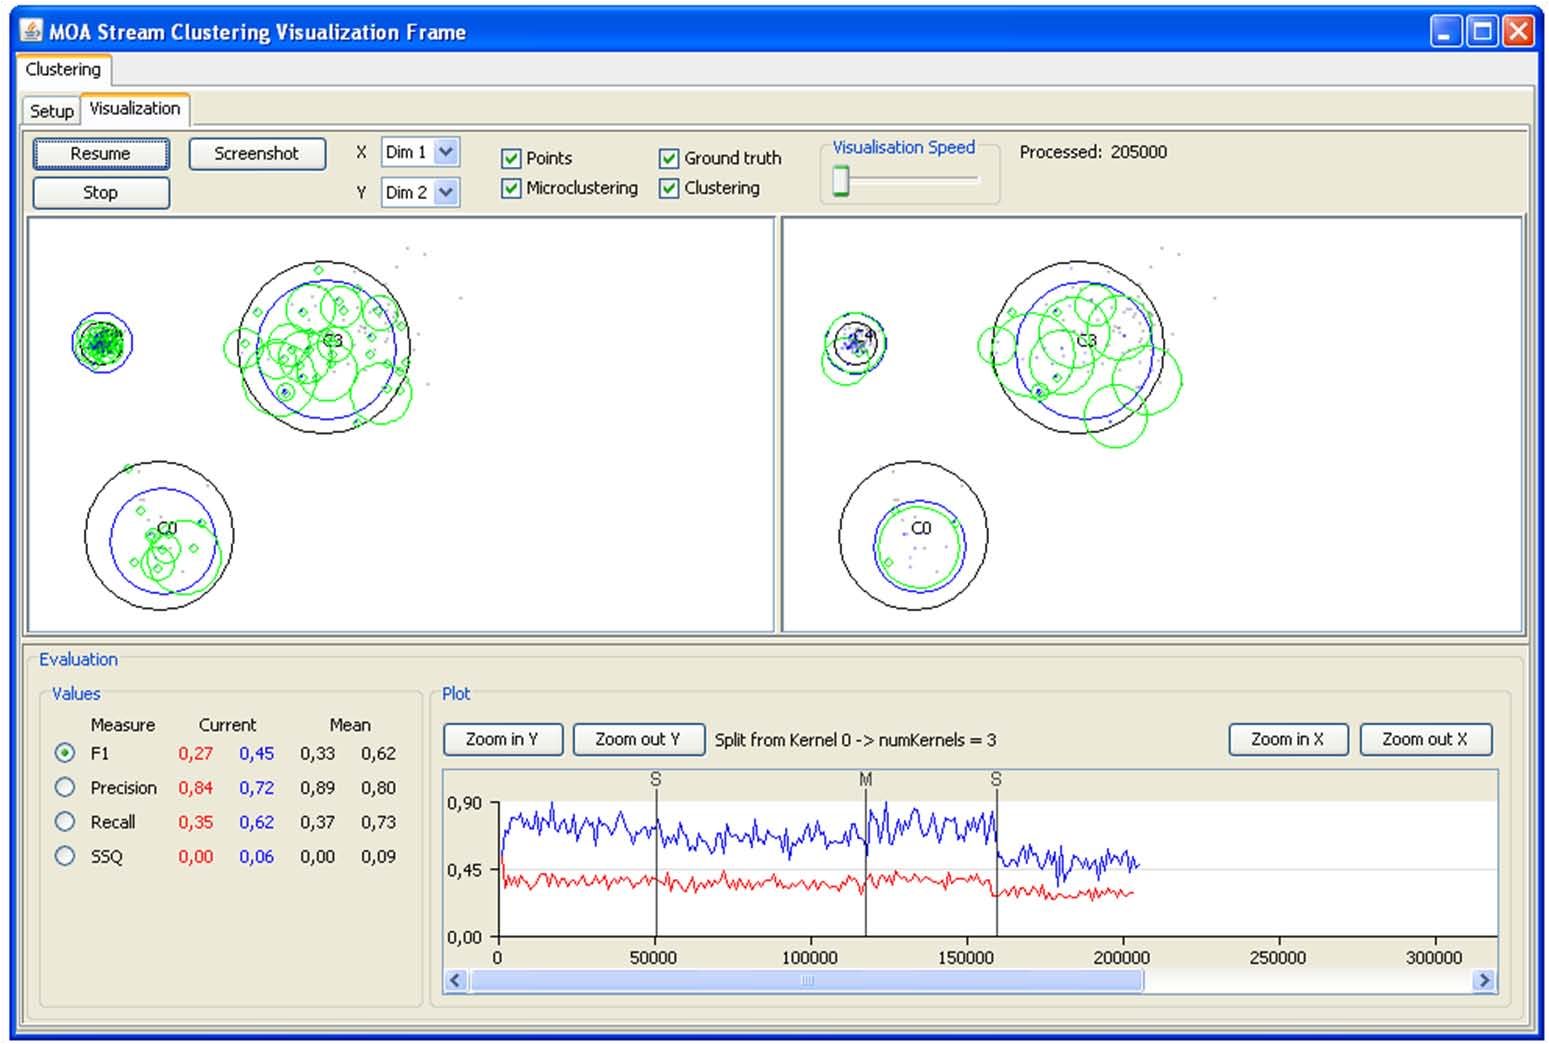
\includegraphics[width=0.8\linewidth]{figures/moa-gui-2.png}
\caption[MOA's Graphical User Interface]{MOA's Graphical User Interface, showing the clustering visualization capabilities of the software.}
\end{figure}

MOA supports bi-directional interaction with WEKA, the Waikato Environment for Knowledge Analysis, which is an award-winning open-source workbench containing implementations of a wide range of batch machine learning methods. WEKA is also written in Java. The main benefits of Java are portability, where applications can be run on any platform with an appropriate Java virtual machine, and the strong and well-developed support libraries. Use of the language is widespread, and features such as the automatic garbage collection help to reduce programmer burden and error.

The MOA framework provides a graphical user interface (GUI), which eases its use, when experiments can be carried out using the algorithms already included in the framework. However, for more complicated analysis or industry-scaled uses, MOA offers the possibility to be used using a command line interface, which is extremely powerful and flexible. Also, due to its open source nature and the fact that it is built in Java, custom procedures and integration techniques can be developed to meet the data analysis requirements. Last but not least, when the core features are not sufficient for the user's needs, MOA can be extended with new mining algorithms, new stream generators or evaluation measures, like the SDC filters that we will implement in this project.
\section{Statistical Disclosure Control software}
\label{State::SDC}



\textbf{Privacy preserving \textit{Stream} Mining:} many of the previously listed methods are already implemented in many classical data mining frameworks and software systems; for example, the \texttt{sdcMicro} package for the \textbf{R} statistical package~\cite{sdcMicro}. However, privacy preserving methods are still not widespread in the stream mining ecosystem - that is another motivation for this project.


\chapter{Practical aspects} % Main chapter title
\label{Chapter4PracticalAspects} % For referencing the chapter elsewhere, use \ref{Chapter1Introduction}
\lhead{\emph{Practical aspects}} % This is for the header on each page - perhaps a shortened title

%----------------------------------------------------------------------------------------

This chapter addresses the \textit{practical} aspects of this project, this is, those that are related to the \textit{praxis}\footnote{\textit{Praxis} is the process by which a theory, lesson, or skill is enacted, embodied, or realised. \textit{Praxis} may also refer to the act of engaging, applying, exercising, realizing, or practicing ideas.}, rather than to technology or theory. An analysis of the concept of privacy and the need to protect it is given in the first section of the chapter, followed by a short review of the legal framework that applies to this project and, finally, a brief note on the environmental impact of the present work.

\section{Privacy \& society}
\label{Practical::Privacy}

Privacy has become a hot topic in debates nowadays, concerning \textit{what} information is collected from individuals, \textit{who} owns it and with \textit{which} purposes. It is a matter of great importance and certainly worth to be examined carefully. Information technologies have brought us many benefits at many levels --- safer streets, cheaper communications, better health systems, more convenient shopping --- but many times at the high cost of losing our privacy. With the rapid adoption of the Internet and all sorts of digital telecommunications as the basis of our modern communication relationships, a vast capacity of interception, storage and analysis of such information exchanges has been reached. This potential has been used by companies in the private sector to, for example, analyze the population consuming profiles, target marketing campaigns more accurately and offer much more customized products and services. In order to apply these techniques and mechanisms, corporations collect private data from users, excusing that these same users accept privacy terms and conditions. It seems clear that data mining is highly related to privacy: knowledge discovery processes need data to work and, in most cases, sensitive personal data is at stake.

We have already outlined in~\sref{Theory:SDC} that the aim of SDC and this project in particular is to protect users privacy by avoiding information disclosure from released datasets and real time analysis processes that require sensitive data. The question, however, is: why do we \textit{need} to protect privacy? What urges us to preserve our right to privacy? It is not a simple and mere question; indeed, the answer is related to our understanding and interpretation of the term ``privacy'' itself. Therefore, we will review the definition of privacy and provide an argument that is the basis to justify privacy protection.

In the introductory chapter of the report (see~\sref{Introduction::Context::Privacy}) an introduction to the concept of privacy was given by literally reproducing a dictionary definition: ``\textit{Privacy is a concept that can be defined as the ability of an individual or group to seclude themselves, or information about themselves, and thereby express themselves selectively}''. We also saw that privacy is recognised as one of our most fundamental rights, as it is enshrined in the Universal Declaration of Human Rights. Going further on, \textit{privacy}, understood not only as the mechanism that allows us to keep our opinion and ideas private, but also the rest of our \textit{praxis}, enables us to develop a \textit{particular} personality, yet when we are within a social structure. Without the right to keep certain aspects of our life private, the \textit{individuation} process is compromised and many consequences of this individual diversity are endangered --- thought heterogeneity, for example, cultural heritage and, above all, individuals \textit{emancipation}, all because the individuation process does not happen in a context of complete freedom.

We must not forget that when organizations such as enterprises or governments acquire massive amounts of private information about particular individuals, a certain \textit{control} capacity on these individuals is gained too. This power, on the contrary of what ultimate defendants of data gathering hold, does not liberate people nor make them more safe. The true consequence of such an increase in control power is that all equitable bonds between individuals and these organisms are torn apart: people become \textit{dominated} by social institutions, be them governments or any kind of structured association, and their freedom is, thus, canceled. There is no possible emancipation nor conviviality of people in a social context if the individuals-society relationships are domain based.

Finally, from a more pragmatic point of view, not only ethical concerns are addressed by protecting users privacy, but economical issues too. Industrial-scale information theft has a huge impact on enterprise economies, because of distrust and because disclosed sensitive data can be used to make profit of it. Identity theft, for example, was estimated to have a cost in the order of billions of dollars, back in 2005, as shown by~\citet{Romanosky:DisclosureLaws}.

\subsection{Impact of this project}
\label{Practical::Privacy:Impact}

The motivation of the project is now well-founded: privacy is a relevant concern for any data analysis related field, it is statistics, data mining or data stream processing. Of course, this project addresses just a small portion of a broader picture, but it is indeed another effort taken towards the effective privacy protection we strive for.

Together with good IT security practices, a reasonable usage of data and information and ackowledged consent from the data owners, the application of SDC techniques --- like the ones implemented by the privacy filters which conform the goal of this project --- enables the preservation of the inalienable right to privacy.

To provide further examples of the impact of the project, potential users of the MOA privacy filters are both companies and government statistical agencies, which handle vasts amounts of sensitive and personal data. Using SDC methods, they would be able to exploit intrinsic knowledge of these data, while preserving privacy and protecting their users against disclosure attacks. Not only they could carry more interesting experiments, but they could also release this information, sharing it with third parties to promote collaboration with researchers and, last but not least, as an exercise of transparency.
\section{Legal framework}
\label{Practical::Legal}

\section{Environmental issues}
\label{Practical::Environmental}

No relevant direct environmental impact is related to this project, neither tied to its
development nor its further deployment. No use of massive resources is done and the
results of the work will not, presumably, result in a significant environmental change of
any kind.

It is still true, however, that data mining, as a discipline and its broad use, does
consume a lot of resources, in terms of technological infrastructure and energy. We cannot
forget that collecting, storing and processing data at the industry scale needs entire data
centers fully dedicated to the data mining process. Power consumption is a big concern
with nowadays information technology, as it is the huge amount of rare materials that
electronic devices contain. These are derived or indirect effects of the data mining process.
This issue deserves to be examined more closely, in the project’s final report.


\chapter{Project management} % Main chapter title
\label{Chapter5ProjectManagement} % For referencing the chapter elsewhere, use \ref{Chapter1Introduction}
\lhead{\emph{Project management}} % This is for the header on each page - perhaps a shortened title

%----------------------------------------------------------------------------------------

This chapter discusses all the aspects concerning the management of the project: \textit{scope}, \textit{schedule} and \textit{budget}. However, we must stress that this classical approach of management analysis is not really suited for our needs. Instead, a more \textit{Agile}\footnote{Agile software development is based on the \textit{Agile manifesto}~\cite{web:AgileManifesto}.} methodology will be applied. We cover this on the~\nameref{Management:Methodology} section, but there is an important conceptual change to be taken into account: the different driving force of the project. Whereas in classical project management the scope-schedule-budget triad is what must be controlled, in an Agile project management approach it is \textit{value}. Indeed, \textit{quality} must be ensured so maximum value is delivered to the project's stakeholders, thus being scope, cost and schedule just \textit{secondary} constraints to these primary goals.

\begin{figure}[ht]
	\centering
	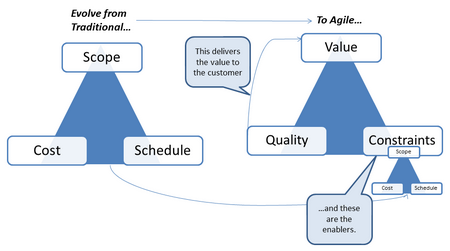
\includegraphics[width=0.7\linewidth]{figures/agile-triangle.png}
	\caption[Transitioning to Agile methodologies.]{Traditional to Agile project management evolution. Source: Agile Australia - Opening keynotes~\citep{web:AgileTriangle}}
	\label{fig:agile-pm}
\end{figure}

\section{Goals \& scope}
\label{Management:Scope}

One of the first things to do when beginning any project is delimiting its \textbf{scope}, this is, deciding \textit{what} will be done and \textit{how}, in terms of resources and methodology.

We already stated in \sref{Introduction::moa-ppsm} what the main \textit{goal} of this project is:

\begin{quote}
	\begin{description}
		\item[Main goal:] \hfill \\
		Implement privacy preserving filters for the Massive Online Analysis (MOA) stream mining framework.
	\end{description}
\end{quote}

\subsection{Requirements analysis}
\label{Management:Scope:Requirements}

For the sake of completeness and verbosity, a more detailed list of the project's \textit{requirements} is given in the next couple of sections, categorized into \textit{functional}\footnote{Functional requirements explain what has to be done by identifying the necessary task, action or activity that must be accomplished.} and \textit{non-functional}\footnote{Non-functional requirements are requirements that specify criteria that can be used to judge the operation of a system, rather than specific behaviors.} ones. Together, they comprise the formal scope of the project.

\subsubsection*{Functional requirements}

\begin{enumerate}[leftmargin=1.5cm, label=\textbf{R\arabic*}]
	\item
	Implement privacy preserving stream mining \textit{filters}\footnote{Within the MOA context, \textit{filters} are procedures applied to data prior to their analysis using machine learning algorithms.} for the MOA stream mining framework. The \textit{suggested} algorithms to be implemented correspond with the following requirements:
	\begin{enumerate}[label*=\textbf{-\arabic*}]
		\item Noise addition~\citep[p.~54]{Hundepool:StatisticalDisclosureControl}
		\item Multiplicative noise~\citep[p.~57]{Hundepool:StatisticalDisclosureControl}
		\item Microaggregation~\citep[p.~60]{Hundepool:StatisticalDisclosureControl}
		\item Rank swapping~\citep[p.~73]{Hundepool:StatisticalDisclosureControl}
		\item Differential privacy~\citep{Dwork:DifferentialPrivacy}
	\end{enumerate}
	
	\item
	Evaluate technological alternatives prior to the implementation of the privacy filters.
	
	\item
	Benchmark the performance of the filters in terms of \textit{disclosure risk} and \textit{information loss}.
\end{enumerate}

\subsubsection*{Non-functional requirements}

\begin{enumerate}[leftmargin=1.5cm, label=\textbf{NFR\arabic*}]
	\item
	\textit{Correctness:} privacy protection is at stake in this project, so algorithms must be implemented correctly, from the theoretical point of view, in order to not ease information disclosure when they are used.
	
	\item
	\textit{Efficiency:} given that no data mining process can scale well if its algorithms are slow, effort will be put in making them the most efficient we can.
	
	\item
	\textit{Test coverage:} measures and tests will be performed to assess the quality of the developed software, as well as its scalability and performance, which is paramount in this project’s context.
	
	\item
	\textit{Documentation:} MOA is an \textit{open source} data mining framework, which means that its community can assess how is it built and how to improve it. One of the benefits of the open source development model is that software can be safer, more robust and efficient, by receiving contributions from different developers. If people are to continue improving the work done, it has to be well documented.
\end{enumerate}

\subsection{Scope deviations}
\label{Management:Scope:Deviations}

There have been no major changes in the scope of the project along its development. Both the functional and non-functional requirements sets remain the same as the ones defined in the final report of the Project Management course (and also listed above).

However, concerning its completion, we have to admit that not all requirements have been achieved. We provide now an enumeration of the functional requirements and their final status:

\begin{enumerate}[leftmargin=1.5cm, label=\textbf{R\arabic*}]
	\item
	\textsc{[Mostly completed]} Implement privacy preserving stream mining \textit{filters} for the MOA stream mining framework.
	\begin{enumerate}[label*=\textbf{-\arabic*}]
		\item \textsc{[Completed]} Noise addition~\citep[p.~54]{Hundepool:StatisticalDisclosureControl}
		\item \textsc{[Not completed]} Multiplicative noise~\citep[p.~57]{Hundepool:StatisticalDisclosureControl}
		\item \textsc{[Completed]} Microaggregation~\citep[p.~60]{Hundepool:StatisticalDisclosureControl}
		\item \textsc{[Completed]} Rank swapping~\citep[p.~73]{Hundepool:StatisticalDisclosureControl}
		\item \textsc{[Completed]} Differential privacy~\citep{Dwork:DifferentialPrivacy}
	\end{enumerate}
	
	\item
	\textsc{[Completed]} Evaluate technological alternatives prior to the implementation of the privacy filters.
	
	\item
	\textsc{[Completed]} Benchmark the performance of the filters in terms of \textit{disclosure risk} and \textit{information loss}.
\end{enumerate}

Even though the \textbf{R1-2} requirement could not be finished, and further work would be possible, as will be discussed in the Conclusions section, the Agile approach for this project has enabled us to avoid a sense of failure at the end of its development.
\section{Methodology}
\label{Management:Methodology}

The methodology approach used in this project will be based on Agile principles. Some of the key concepts and practices related to Agile software development are:

\begin{itemize}
	\item \textbf{Iterative} development versus the classical \textit{waterfall} development model.
	\item Short to mid range development \textbf{sprints} (phases), in order to keep track of the project’s evolution and to be able to react to changes, unforeseen constraints or scope drifts.
	\item \textbf{Constant meetings} with the project’s stakeholders, in which the progress and deviations of the project are assessed.
	\item Usage of \textbf{burndown charts} - a graphical model of work left to do versus time - and other visual representations of the project's track
	\item Reduced documentation generation, to alleviate the potential loss of time that changes in the requirements would cause.
\end{itemize}

Among many other approaches and Agile methodological frameworks, \textit{Scrum} is one of the most well-known due its flexibility, its proved resilience against requirements rapid changes and easy adoption by software development teams.

\subsection{Scrum}

\textbf{Scrum} is an iterative and incremental agile software development methodology for managing product development. It challenges assumptions of the \textit{traditional, sequential approach} to product development, and enables teams to self-organize by encouraging physical location or close online collaboration of all team members, as well as daily face-to-face communication among all team members and disciplines in the project~\citep{web:Wiki:Scrum}.

\begin{figure}
	\centering
	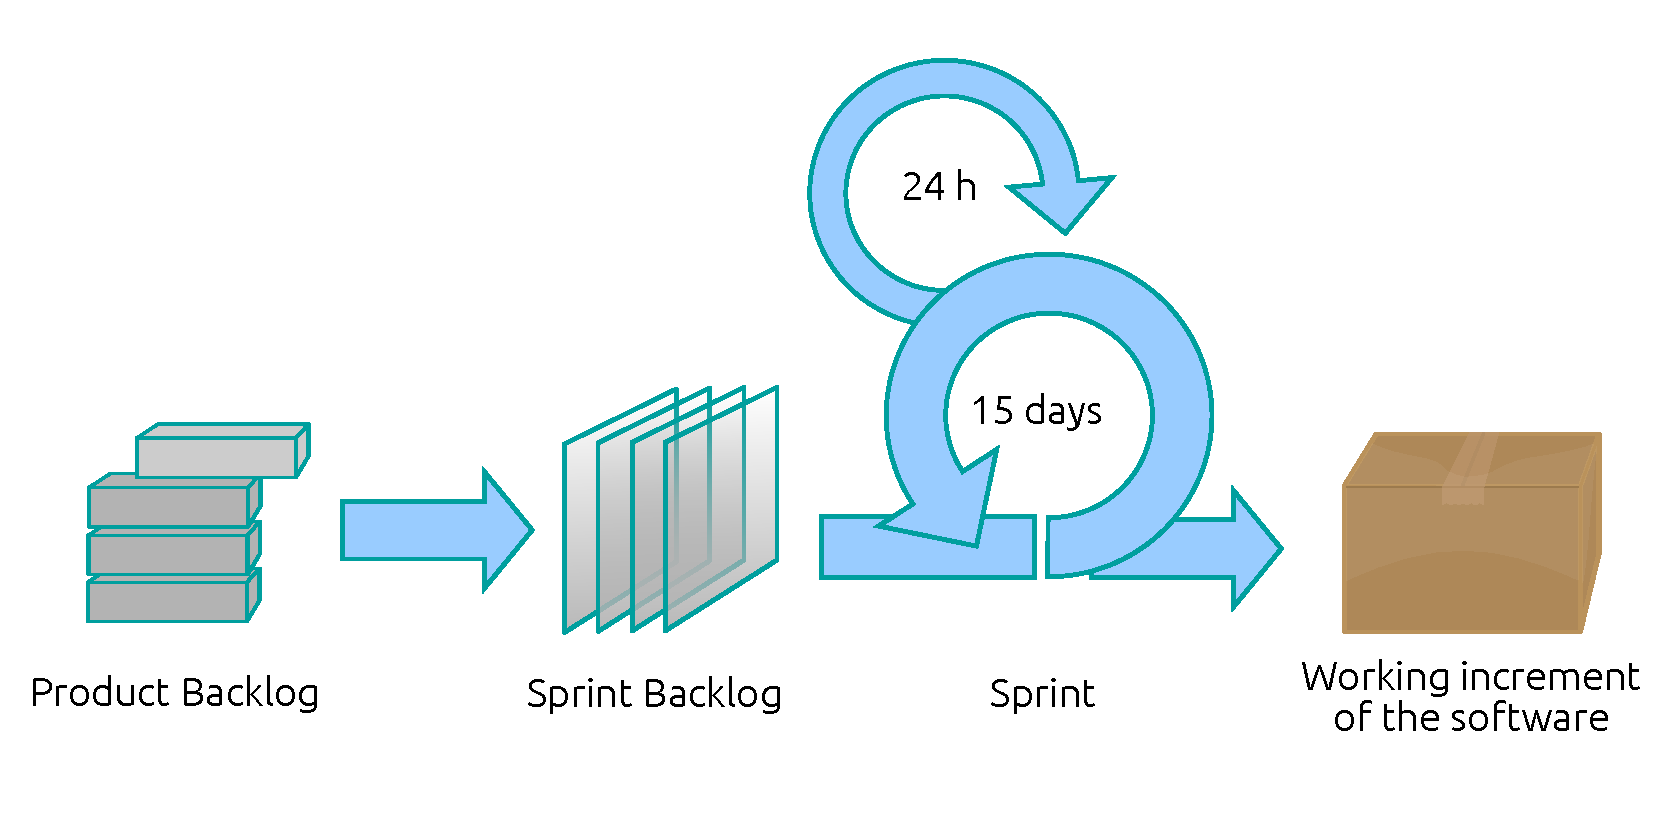
\includegraphics[width=0.8\linewidth]{figures/scrum.pdf}
	\caption{\textit{Scrum} methodology process overview. Adapted from Wikimedia~\citep{web:Wiki:ScrumProcess}}
	\label{fig:scrum}
\end{figure}

This methodology is based on the adoption of certain roles, as well as some \textit{artifacts} and predefined processes, all of which can be adapted as necessary by the team to suit their specific needs and resources. However, a central concept forms the basis for the rest of the framework: the \textbf{sprint}. A sprint or iteration is the basic unit of development in Scrum. The sprint is a timeboxed effort, this is, it is restricted to a specific duration, which is fixed in advance for each sprint and is normally between one week and one month, with two weeks being the most common.

\subsubsection*{Roles}

The follwing are the relevant roles that emerge in a Scrum developed project:

\begin{itemize}
	\item
	\textbf{Product owner:} the product owner represents the stakeholders and is the voice of the customer. He or she is accountable for ensuring that the team delivers value to the business. The product owner writes \textit{user stories} (tasks) and adds them to the \textit{product backlog}, prioritizing them.
	
	\item
	\textbf{Scrum master:} Scrum is facilitated by a scrum master, who is accountable for removing impediments to the ability of the team to deliver the product goals and deliverables. The scrum master is not a traditional team lead or project manager, but acts as a buffer between the team and any distracting influences. The scrum master ensures that the scrum process is used as intended.
	
	\item
	\textbf{Development team:} the development team is responsible for delivering potentially shippable increments of product at the end of each \textit{sprint}. A team is made up of 3–9 individuals with cross-functional skills who do the actual work: analyse, design, develop, test, document, etc. Finally, it is important to emphasize that the development team in Scrum is self-organizing.
\end{itemize}

\subsubsection*{Events}

A series of \textit{events} take place during the Scrum process, configuring the actual workflow of the team. We will provide an overview of some of them:

\begin{itemize}
	\item
	\textbf{Sprint planning:} at the beginning of a sprint, the team holds a sprint planning event, in which the work to be done is selected from the product backlog and transferred to the sprint backlog.
	
	\item
	\textbf{Daily Scrum:} a stand-up, timeboxed and short meeting takes place every day during each sprint. In these meetings, every member of the team explains the work carried out the previous day, discusses any impediment or blocking situation he or she has encountered and decides which tasks will do in the following day.
	
	\item
	\textbf{Retrospective:} at the end of each sprint, a review of the work that has been completed is made, and the team reflects on the past sprint to identify and agree on any process improvement, which requires actions to be taken in the upcoming sprint.
\end{itemize}

\subsubsection*{Artifacts}

Even though we have given an overview of some of them, the following artifacts are the remaining pieces that shape up the Scrum process and methodology:

\begin{itemize}
	\item
	\textbf{Product backlog:} the product backlog is an ordered list of requirements that is maintained for a product. It consists of features, bug fixes, non-functional requirements, etc., i.e., whatever needs to be done in order to successfully deliver a viable product. The items in this backlog are ordered by the product owner based on considerations like risk, business value, dependencies or date needed, for example.
	
	\item
	\textbf{Sprint backlog:} The sprint backlog is the list of work the development team must address during the next sprint. The list is derived by selecting product backlog items from the top of the product backlog until the development team feels it has enough work to fill the sprint. The development team should keep in mind its past performance assessing its capacity for the new sprint, and use this as a guide line of how much \textit{effort} they can complete.
\end{itemize}

\subsection{Agile in this project}

The methodology chosen for this project will be based upon Scrum, but major modifications will have to be made, for a number of reasons. Firstly, there is no such \textit{development team}: a single developer will take care of the implementation of the project. Moreover, there is no possibility of having a Scrum master either. The project director will take a role between a technical coordinator and a product owner, although no real concept of \textit{product} exists in the project, either way.

\subsubsection{Practices}

The adopted Agile practices for this project include:

\begin{itemize}
	\item The usage of Trello\footnote{Its description, along with other resources and tools used, can be found on~\sref{Management:Budget:Resources}} as a task tracking tool, to prioritize them similarly to the Scrum backlogs.
	\item \textbf{Sprint}-based development cycles with a sprint duration of one week.
	\item Constant (re)-evaluation of constraints and requirements, to forsee changes and take preventive action (similar to retrospectives, but less formal and certainly shorter).
\end{itemize}

\subsubsection{Scope}

Adopting Agile methodologies involves several decisions on how to manage the project and its requirements. In this particular project, if we are to examine the classical constraints (of which we talked about at the beginning of this chapter), we must be aware that the \textit{schedule is fixed} (perhaps not the planning, but the final milestone) and this forces us to let the \textbf{scope opened}. This means that we will implement as much features as we can, assessing their quality, but no feature list will drive the success or failure of the project. Because we will be working on the basis of such an \textit{open scope}, deviations in this field are likely to happen. These, however, will not result in a project failure in any case, because an agreement has been reached to work this way.
\section{Schedule}
\label{Management:Schedule}

The following subsections provide some details about the initial project planning (\sref{Management:Schedule:Initial}), as well as the changes it has suffered over time (\sref{Management:Schedule:Final}). There have been \textit{significant} deviations concerning the original project schedule. Not only the global duration has been lengthened, but more phases have been layed out, as was needed. As a positive contrast, early detection of such alterations has been sometimes possible.

\subsection{Initial schedule}
\label{Management:Schedule:Initial}

In this section, we cover the original analysis that was reported during the Project Management module\footnote{The Project Management module is a compulsory course that all students have to undertake when beginning their Bachelor's Degree Final Project, concerning project management concepts and techniques, as well as documentation.}, at the beginning of this project's development.

\subsubsection{Overall duration}

Taking a general look at the project’s schedule, we can estimate it to have a total duration of about 5 months. Even though it was registered on July, 2014, the project did not begin until September, because August is the only month I can have holidays, due to job restrictions. Considering the next possible project’s lecture shifts, we believe that the one taking place in December is too close in time. Thus, the project will endure until January the 26th, 2015. This should give us time enough to develop the project and document it without too much pressure, which is key to fulfill one of the main established goals: high quality results.

\subsubsection{Schedule slack}

The project schedule we present herein does not fill up the total amount of time available - more than two weeks are left blank, with no assigned tasks. This is intended because of the following reasons:

\begin{itemize}
	\item The amount of time needed to develop the proposed algorithms is uncertain. It is hard to estimate the time it may take, because I have no previous knowledge on the area. Therefore, we opted for, in one hand, an \textit{open scope} approach, and, on the other, leaving a considerable time gap between the last planned task and the project’s final milestone: its defense. Being conservative, if the development of any proposed method is delayed, we still have some leeway to introduce schedule changes, without risking the project’s success.
	
	\item We have estimated the project’s report confection and the defense presentation rehearsals to be 35 and 7 days, respectively, but depending on how much development is finally carried out, it might not be time enough to write down the report. Extra time for doing it can be then borrowed from the schedule slack time.
	
\end{itemize}

\subsubsection{Schedule monitoring \& changes}

For the development phase of the project, the most suitable way to monitor the schedule we have found is applying an Agile approach to the process. We will work in one week long sprints, meeting every week to assess the quality of the solutions, the proper progress of the project and to plan what will be done during the following sprint.

Sprint planning meetings are where the main goals of the project will be sliced in small tasks, which can be tracked and implemented better, because they are not so complex. Thanks to this constant fine-grained planning process, schedule or scope deviations are detected earlier and can be managed efficiently, reacting before they affect deeper the overall success of the project. Given that no fixed features list is assigned to each sprint of the development phase, if the completion of either of those features is delayed, it can be made to span for some more time.

Within each of the development sprints, burndown charts\footnote{A burn down chart is a graphical representation of work left to do versus time. The outstanding work (or backlog) is often on the vertical axis, with time along the horizontal. That is, it is a run chart of outstanding work. It is useful for predicting when all of the work will be completed. It is often used in agile software development methodologies such as Scrum.} will be used to monitor the progress of the sprint. These charts are helpful in identifying patterns of work (sprint-end rushes, for example) and can help developers maintain a constant rate of finished features.

Besides burndown charts and sprint planning meetings, the use of velocity charts will also be helpful to increase the predictability of the following sprint plannings. The more predictable they are, the less deviations will occur and the schedule will be more likely to be fulfilled.

\subsubsection{Project phases}

The project is divided in 4 main phases, besides of the undertaking of the Project's Management module. Each phase has an estimated duration and a risk evaluation in terms of schedule deviation. The amount of hours is an approximated calculation from the number of days in each phase: 4 hours a day are estimated to be spent, because I am currently working part-time and also taking some subjects. A more detailed task granularity can be seen in the Gantt chart (on \fref{fig:gantt-1} and~\fref{fig:gantt-2}). Task dependencies are shown in the chart too. Those phases, chronologically ordered are:

\begin{enumerate}[leftmargin=1.5cm, label=\textbf{{[}Phase \arabic*{]}}]
	\item \textbf{Contextualization}: it is intended to perform a deeper bibliographic research and a study of the main subjects concerning the project, at the theory level - no practical skills or technological research will be done.
	\begin{itemize}
		\item \textbf{Duration estimation:} 11 days (44 hours).
		\item \textbf{Risk:} this phase has a medium to high risk of being delayed, due to lack of effective time (a wrong estimation), and also because more insight than planned might be needed, consuming more time.
	\end{itemize}
	
	\item \textbf{Environment setup}: during this phase, all necessary tools and material resources will be gathered and configured. The concrete developing workflow will be decided, too.
		\begin{itemize}
			\item \textbf{Duration estimation:} 8 days (32 hours).
			\item \textbf{Risk:} this phase has a low risk of being delayed, because the technology that is to be used is, a priori, well known to us.
		\end{itemize}
		
	\item \textbf{Development}: all of this project coding will be performed during this phase. As said before, a sprint methodology will be used during this phase, being one week each.
		\begin{itemize}
			\item \textbf{Duration estimation:} with an initial planning of 7 sprints, 49 days will be used (196 hours).
			\item \textbf{Risk:} there is a medium risk of this phase to be delayed. Even with the use of Agile methodologies, if a fundamental feature was needed and there was no more time left, another sprint (or at most a couple of them) could be introduced, to finish the remaining tasks.
		\end{itemize}
		
	\item \textbf{Documentation}: the project’s report will be written after the development phase, along with any deployment documentation that was required and the final presentation, which will also be rehearsed then.
		\begin{itemize}
			\item \textbf{Duration estimation:} 42 days (168 hours).
			\item \textbf{Risk:} this phase has a medium risk of being delayed too. Reviews of the report will be made and writing in English might take up more time than expected.
		\end{itemize}
	
\end{enumerate}

\subsubsection{Detailed schedule: Gantt chart}

A detailed Gantt chart of the schedule can be seen in~\fref{fig:gantt-1} and~\fref{fig:gantt-2}. The chart was generated with the \textit{Project management} free software package, available online on the Ubuntu 12.04 Software Center. Please note that there is no way the chart could fit in a single page (not even if it was landscape).

\begin{figure}[hbtp]
	\makebox[\textwidth]{
		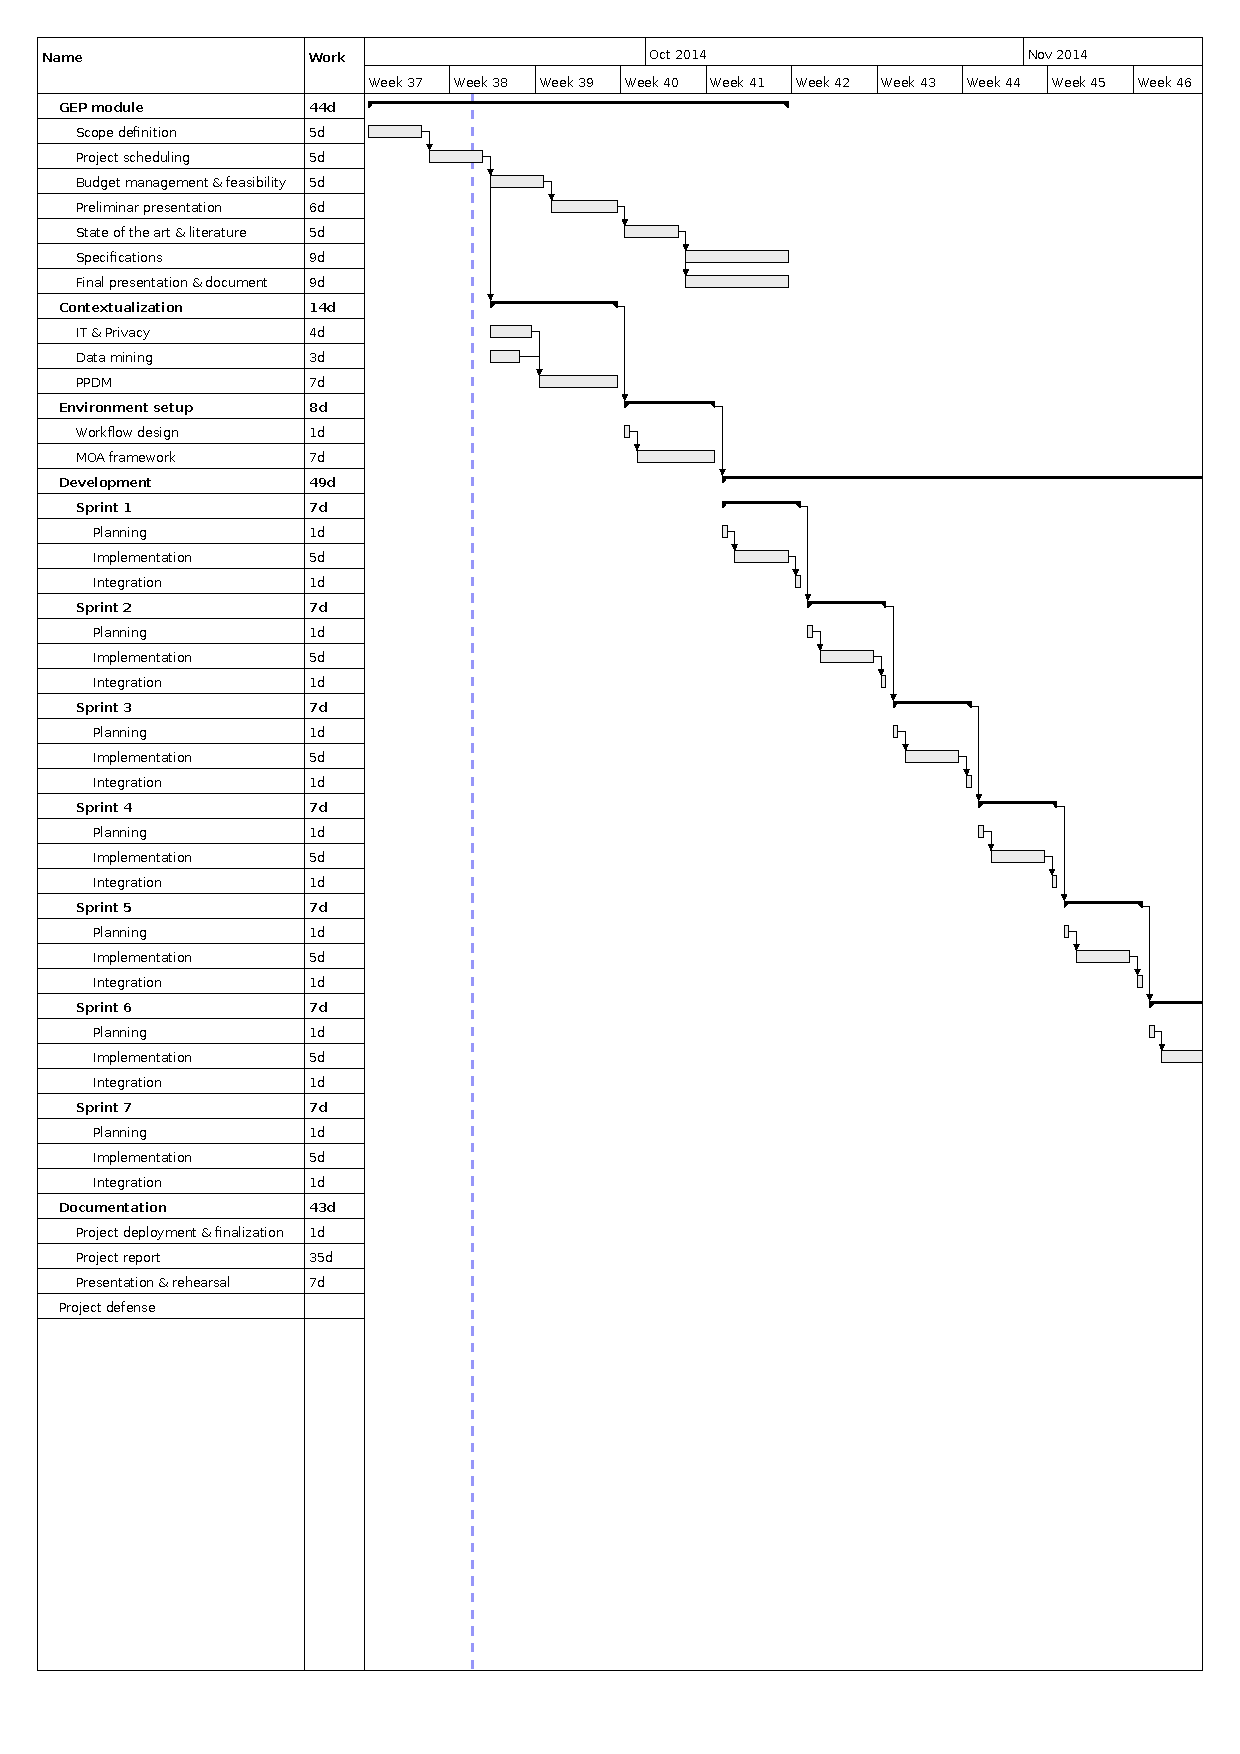
\includegraphics[trim={0 7.3cm 0 0},clip,page=1,width=1.2\linewidth]{figures/gantt-chart.pdf}
	}
	\caption{Initial project schedule Gantt chart (part 1).}
	\label{fig:gantt-1}
\end{figure}

\begin{figure}[hbtp]
	\makebox[\textwidth]{
		\includegraphics[trim={0 7.3cm 0 0},clip,page=2,width=1.2\linewidth]{figures/gantt-chart.pdf}
	}
	\caption{Initial project schedule Gantt chart (part 2).}
	\label{fig:gantt-2}
\end{figure}

\clearpage

\subsection{Schedule deviation}
\label{Management:Schedule:Final}

We will cover now the changes that have occurred in the schedule of the project and analyze its causes.

\subsubsection{Overall duration}

The original total duration has been extended from 5 months to 8 months, approximately. Thus, the final report and its defence is now scheduled to be in April, which is the next available lecture shift in the Faculty. We believe that this extended duration will allow us to fulfill all requirements defined in the scope of the project.

\subsubsection{Deviation analysis}

There are several possible reasons behind this schedule deviation:

\begin{itemize}
	\item The Project Management module lasted longer than expected, forcing the development phase of the project to begin later.
	\item During the definition of the project initial schedule, we expected to begin developing it while the Project Management module endured, which was, definitely, a planning error. Such tasks concurrency was not possible at that time.
	\item At the beginning of the development phase, we explored different technological alternatives, before deciding which approach was mostly suited to our needs, but this exploration delayed the actual development process for a couple of weeks.
	\item As was already stated in the Project Management report, some of the requested features have posed to be more complicated than was expected, consuming some more time than that assigned to them.
	\item For personal reasons, no work could be carried out during the Christmas vacations, which lasted two more weeks, furtherly delaying the project's development.
\end{itemize}

\subsubsection{Current detailed schedule}

Considering the previous analysis, a new Gantt chart has been built, with the new project's schedule, which is detailed in~\fref{fig:new-gantt-1} and~\fref{fig:new-gantt-2}.

\begin{figure}[hbtp]
	\makebox[\textwidth]{
		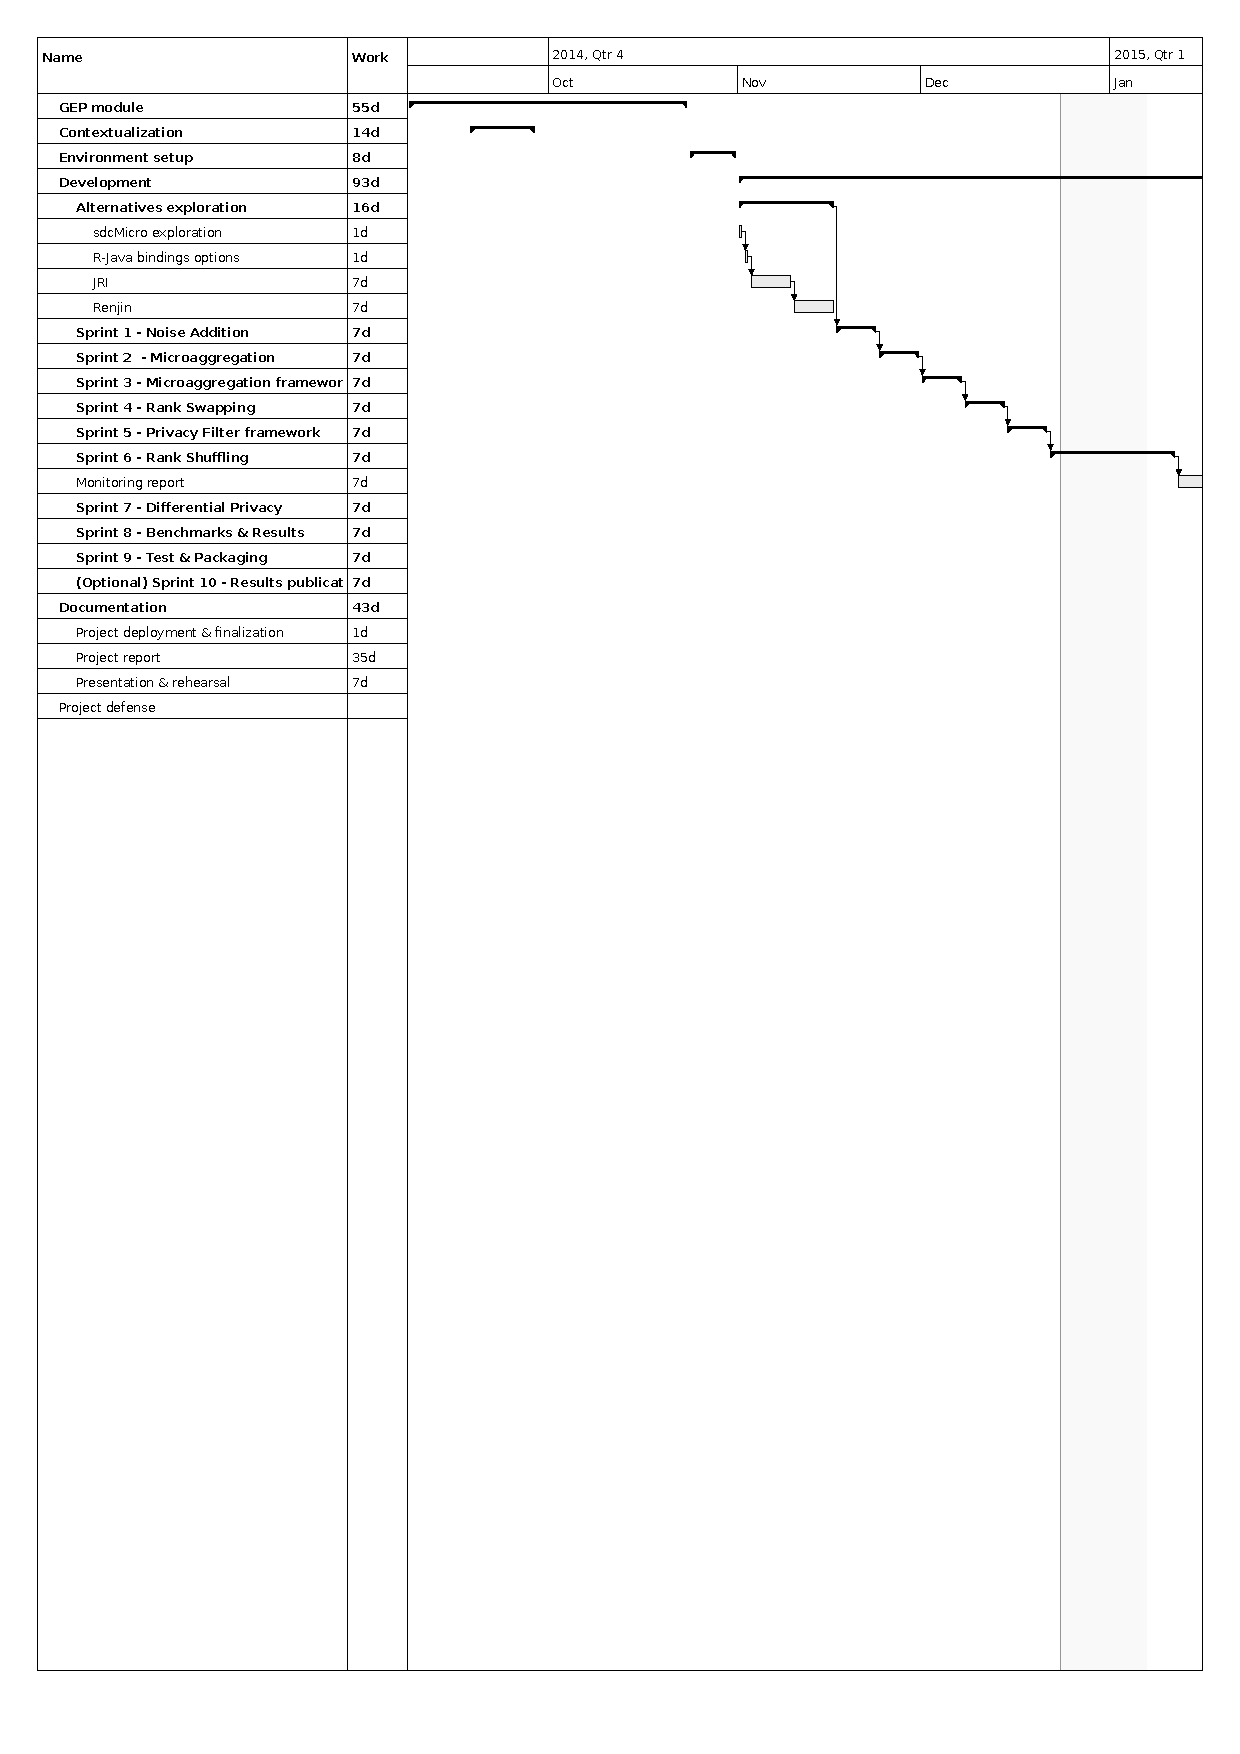
\includegraphics[angle=90,trim={0 17.5cm 0 0},clip,page=1]{figures/new-gantt-chart.pdf}
	}
	\caption{Final project schedule Gantt chart (part 1).}
	\label{fig:new-gantt-1}
\end{figure}

\begin{figure}[hbtp]
	\makebox[\textwidth]{
		\includegraphics[angle=90,trim={0 17.5cm 0 0},clip,page=2]{figures/new-gantt-chart.pdf}
	}
	\caption{Final project schedule Gantt chart (part 2).}
	\label{fig:new-gantt-2}
\end{figure}

\clearpage
\section{Budget}
\label{Management:Budget}

The initial budget and resources analysis, performed during the Project Management module, corresponds with~\sref{Management:Budget:Resources},~\sref{Management:Budget:Estimation} and~\sref{Management:Budget:Control}. Due to schedule deviations during the project, a final budget estimation is given in~\sref{Management:Budget:Final}.

The project’s budget is entirely based on an estimation of human, hardware and software resources costs. No real income is perceived, besides the salary of the project’s supervisor, who is a tenure-track lecturer at the Barcelona School of Informatics, and an associate researcher at the Barcelona Supercomputing Center. No third parties are involved in the project - no companies or organizations are providing any funds. Moreover, even though the work is to be integrated into the MOA framework, it is indeed an open-source project, to which we will be contributing, meaning contributions are expected from any kind of source, be it funded or not.

All other associated costs are \textit{externalized}, either by people involved in the project or by the university, where the development of the project will be held.

\subsection{Resources \& budget estimation}
\label{Management:Budget:Resources}

Resources consumed in this project only fall in one of the following categories: \textit{human resources}, \textit{hardware}, \textit{software} and \textit{other expenses}. For a detailed description of what will be needed in the project, please see the following subsections. It is important to keep in mind that \textit{all} resources will be consumed equally througout the entire project duration.

\subsubsection{Human resources}

Human resources are summarized in~\tref{table:human-resources}.

All expenses included here are related to people’s salaries. Only one developer will be working on this project, but a number of hours involving supervision tasks is also imputed to the project’s supervisor, so its corresponding cost is added too. Taxes are included in all of the following items. The price is also an estimation: on the developer’s side, it is based on a salaries comparison webpage (\textit{Glassdoor}~\citep{web:Glassdoor})\footnote{As of date 12th October, 2014, the average salary for a software engineer in Barcelona is 32000€ per year (including taxes). Considering 12 monthly instalments and an average of 160 hours per month, this yields a total of 16.66€ per hour.}; on the supervisor side, the price is based on his own estimation.

\begin{itemize}
	\item \textbf{Developer:} an average of 20 hours a week are estimated, spanning for about 21 weeks, summing up a total of 420 hours.
	\item \textbf{Supervisor:}
	\begin{itemize}
		\item \textbf{Project’s take off:} 8 hours, between meetings and initial planning.
		\item \textbf{Sprints:} 8 hours each sprint, taking into account both face to face meetings and other supervising tasks. There are 7 sprints scheduled so far, making a total of 56 hours.
		\item \textbf{Documentation:} during the project’s final stage, an estimation of 20 hours is taken from the corresponding supervision of the project’s report.
	\end{itemize}
\end{itemize}

\begin{table}[h]
	\centering
	\begin{tabular}{lllr}
		\hline
		\textbf{Role} & \textbf{Price (per hour)} & \textbf{Working  hours} & \multicolumn{1}{l}{\textbf{Total}} \\ \hline
		Supervisor & \multicolumn{1}{r}{35€} & \multicolumn{1}{r}{84} & 2940€ \\
		Developer & \multicolumn{1}{r}{16.66€} & \multicolumn{1}{r}{420} & 6997.2€ \\ \hline
		&  & \multicolumn{1}{r}{\textbf{Total}} & \textbf{9937.2€}
	\end{tabular}
	\caption{Human resources associated costs. All taxes are included in the Price per hour column.}
	\label{table:human-resources}
\end{table}

\subsubsection{Hardware resources}

Hardware resources are summarized in~\tref{table:hardware-resources}.

All hardware needed resources are shown in the corresponding table. Their cost is calculated by estimating its amortization, spanned over 5 years (it is a personal laptop). To calculate its amortized cost per hour, we will take into account that this equipment is used throughout the course too, and estimating that 2500 hours of work are carried each year.

\begin{table}[h]
	\centering
	\begin{tabular}{l r r r r r}
		\hline
		\textbf{Product} & \multicolumn{1}{l}{\textbf{Price}} & \multicolumn{1}{l}{\textbf{Units}} & \multicolumn{1}{p{3cm}}{\textbf{Amortized price per hour}} & \multicolumn{1}{l}{\textbf{Work time (hours)}} & \multicolumn{1}{l}{\textbf{Total}} \\ \hline
		Asus k53sv & 650€ & 1 & 0.052€ & 420 & 21.84€ \\ \hline
		&  &  &  & \textbf{Total} & \textbf{21.84€}
	\end{tabular}
	\caption{Hardware amortization costs. All taxes included.}
	\label{table:hardware-resources}
\end{table}

\subsubsection{Software resources}

All software needed to undertake this project is free and, most of it, is open sourced. Despite this, we will include a list of it here, to show what will be used at a finer grain.

\begin{itemize}
	\item \textbf{Ubuntu 12.04}: operating system. Available at: \url{http://www.ubuntu.com/download}.
	\item \textbf{Trello}: online task management tool. Available at: \url{https://trello.com/}.
	\item \textbf{Google Drive}: online, collaborative office software suit, used to create burndown charts (spreadsheets). Available at: \url{https://drive.google.com}.
	\item \textbf{Java SDK}: Java language Software Development Kit. Available at: \url{http://openjdk.java.net}.
	\item \textbf{Eclipse IDE}: integrated development environment package. Available at: \url{https://www.eclipse.org/home/index.php}.
	\item \textbf{Git}: source version control system. Available at: \url{http://git-scm.com/}. Remote code repositories will be hosted at GitHub (\url{https://github.com}) for free.
	\item \textbf{MOA}: Massive Online Analysis, a stream mining framework. Available at: \url{http://moa.cms.waikato.ac.nz}.
	\item \textbf{\LaTeX}: document preparation system. Available at: \url{http://www.latex-project.org}.
\end{itemize}

\subsubsection{Other expenses}

All expenses not covered in the previous sections are detailed in~\tref{table:other-resources}.

\textbf{Please note} that the cost of each item of this section is an estimation. Moreover, even though they are displayed, since no budget is really available, they will be \textit{absorbed} by the university, where most of the work will be carried out.

\begin{table}[h]
	\centering
	\begin{tabular}{lrrr}
		\hline
		\textbf{Product} & \multicolumn{1}{l}{\textbf{Price per month}} & \multicolumn{1}{l}{\textbf{Months}} & \multicolumn{1}{l}{\textbf{Total}} \\ \hline
		Energy & 35€ & 4 & 140€ \\
		Water & 25€ & 4 & 100€ \\
		Heat \& air & 30€ & 4 & 120€ \\
		Internet connection & 40€ & 4 & 160€ \\ \hline
		& \multicolumn{1}{l}{} & \textbf{Total} & \textbf{520€}
	\end{tabular}
	\caption{Uncategorized resources estimated costs. All taxes are included.}
	\label{table:other-resources}
\end{table}

\subsection{Total budget estimation}
\label{Management:Budget:Estimation}

The sum of the subtotals of the previous sections is shown in~\tref{table:total-resources}. Please note that, since taxes are already included in each item appropriately, there is no need to add them here.

\begin{table}[h]
	\centering
	\begin{tabular}{lr}
		\hline
		\textbf{Concept} & \multicolumn{1}{l}{\textbf{Total}} \\ \hline
		Human resources & 9937.2€ \\
		Hardware & 21.84€ \\
		Software & 0€ \\
		Other expenses & 520€ \\ \hline
		\multicolumn{1}{r}{\textbf{Total}} & \multicolumn{1}{l}{\textbf{10479.04€}}
	\end{tabular}
	\caption{Total budget: summation of budget estimations.}
	\label{table:total-resources}
\end{table}

All costs are just estimations and are not covered in any way, with the exception of the supervisor’s salary. This means that, in fact, there is no possible way this project is feasible. However, given that the developer has no salary at all and that all other extra costs are assumed by the university or the developer, the project can be developed normally.

\subsection{Budget control mechanisms}
\label{Management:Budget:Control}

Any budget deviations related to material equipment or software purchases will be monitored in the sprint planning meetings at the beginning of each of those phases during the project. These possible extra costs will be assumed by the developer, since no other source of funds is available.

Another source of budget deviations can be found on the project’s duration. If the schedule is not fulfilled and the project is delayed, extra cost in terms of human resources, hardware amortizations and other expenses would have to be added. They still would be treated as they are in the present analysis, meaning no significant change would occur.

\subsection{Final budget estimation}
\label{Management:Budget:Final}

Due to the deviation in the project's schedule, that was already analyzed in~\sref{Management:Schedule:Final}, an increment in the human resources, external expenses and hardware amortization budget contributions has arised. It is important to note that, given that no proprietary software package has been used, no additional costs might be derived from the lenghtening of the project duration. We will now cover this budget deviation and provide a final estimation of the project cost, which is summarized in~\tref{table:final-total-resources}.

\subsubsection*{Human resources: deviation}

Following the analysis from~\ref{Management:Budget:Resources}, we just have to add the corresponding increment of working hours for both the developer and supervisor.

\begin{itemize}
	\item \textbf{Developer:} an average of 20 hours a week are estimated, spanning for about 32 weeks, summing up a total of 640 hours. However, given that no work was carried during Christmas holidays, the total number of hours should be lowered to, at most, \textbf{600 hours}.
	\item \textbf{Supervisor:}
	\begin{itemize}
		\item \textbf{Project’s take off:} 8 hours, between meetings and initial planning.
		\item \textbf{Sprints:} 8 hours each sprint, taking into account both face to face meetings and other supervising tasks. With 10 sprints of final work, this yields a total of \textbf{80 hours}.
		\item \textbf{Documentation:} during the project’s final stage, an estimation of \textbf{20 hours} is taken from the corresponding supervision of the project’s report.
	\end{itemize}
\end{itemize}

Considering the previous estimation and keeping the same prices per hour of the initial estimation, the following total human resources cost is calculated (see~\tref{table:human-resources-final}).

\begin{table}[h]
	\centering
	\begin{tabular}{lllr}
		\hline
		\textbf{Role} & \textbf{Price (per hour)} & \textbf{Working  hours} & \multicolumn{1}{l}{\textbf{Total}} \\ \hline
		Supervisor & \multicolumn{1}{r}{35€} & \multicolumn{1}{r}{108} & 3780€ \\
		Developer & \multicolumn{1}{r}{16.66€} & \multicolumn{1}{r}{600} & 9996€ \\ \hline
		&  & \multicolumn{1}{r}{\textbf{Total}} & \textbf{13776€}
	\end{tabular}
	\caption{Human resources associated costs (final estimation).}
	\label{table:human-resources-final}
\end{table}

\subsubsection*{Hardware resources: deviation}

The only change in the hardware related costs is the number of working hours devoted to the project, which have a direct impact on the amortization of the equipment.

\begin{table}[h]
	\centering
	\begin{tabular}{l r r r r r}
		\hline
		\textbf{Product} & \multicolumn{1}{l}{\textbf{Price}} & \multicolumn{1}{l}{\textbf{Units}} & \multicolumn{1}{p{3cm}}{\textbf{Amortized price per hour}} & \multicolumn{1}{l}{\textbf{Work time (hours)}} & \multicolumn{1}{l}{\textbf{Total}} \\ \hline
		Asus k53sv & 650€ & 1 & 0.052€ & 600 & 31.2€ \\ \hline
		&  &  &  & \textbf{Total} & \textbf{31.2€}
	\end{tabular}
	\caption{Hardware amortization costs (final estimation).}
	\label{table:hardware-resources-final}
\end{table}

\subsubsection*{Other expenses: deviation}

Given that the amount of months dedicated to the project's development has increased, the estimated cost for the expenses related to the developer's accomodation has to reflect the changes as well.

\begin{table}[h]
	\centering
	\begin{tabular}{lrrr}
		\hline
		\textbf{Product} & \multicolumn{1}{l}{\textbf{Price per month}} & \multicolumn{1}{l}{\textbf{Months}} & \multicolumn{1}{l}{\textbf{Total}} \\ \hline
		Energy & 35€ & 7 & 245€ \\
		Water & 25€ & 7 & 175€ \\
		Heat \& air & 30€ & 7 & 210€ \\
		Internet connection & 40€ & 7 & 280€ \\ \hline
		& \multicolumn{1}{l}{} & \textbf{Total} & \textbf{910€}
	\end{tabular}
	\caption{Uncategorized resources estimated costs. All taxes are included.}
	\label{table:other-resources-final}
\end{table}

\clearpage

\subsubsection*{Final estimation}

The following is the final estimation of the project's budget, taking into account all deviations from the particular budget contributions.

\begin{table}[h]
	\centering
	\begin{tabular}{lr}
		\hline
		\textbf{Concept} & \multicolumn{1}{l}{\textbf{Total}} \\ \hline
		Human resources & 13776€ \\
		Hardware & 31.2€ \\
		Software & 0€ \\
		Other expenses & 910€ \\ \hline
		\multicolumn{1}{r}{\textbf{Total}} & \multicolumn{1}{l}{\textbf{14717.2€}}
	\end{tabular}
	\caption{Total budget final estimation.}
	\label{table:final-total-resources}
\end{table}

%----------------------------------------------------------------------------------------
%	THESIS CONTENT - APPENDICES
%----------------------------------------------------------------------------------------

\addtocontents{toc}{\vspace{2em}} % Add a gap in the Contents, for aesthetics

\appendix % Cue to tell LaTeX that the following 'chapters' are Appendices

% Include the appendices of the thesis as separate files from the Appendices folder
% Uncomment the lines as you write the Appendices

% Appendix A

\chapter{Appendix Title Here} % Main appendix title

\label{AppendixA} % For referencing this appendix elsewhere, use \ref{AppendixA}

\lhead{Appendix A. \emph{Appendix Title Here}} % This is for the header on each page - perhaps a shortened title

Write your Appendix content here.
%\input{Appendices/AppendixB}
%\input{Appendices/AppendixC}

\addtocontents{toc}{\vspace{2em}} % Add a gap in the Contents, for aesthetics

\backmatter

%----------------------------------------------------------------------------------------
%	BIBLIOGRAPHY
%----------------------------------------------------------------------------------------

\label{Bibliography}

\lhead{\emph{Bibliography}} % Change the page header to say "Bibliography"

\nocite{*}
\bibliographystyle{unsrtnat} % Use the "unsrtnat" BibTeX style for formatting the Bibliography
\bibliography{bibliography} % The references (bibliography) information are stored in the file named "Bibliography.bib"

\end{document}
